\documentclass[11pt,a4paper]{article}

% Graphviz emits PDF 1.7 figures; match it so their inclusion is silent.
\pdfminorversion=7

\usepackage[margin=1in]{geometry}
\usepackage{amsmath}
\usepackage{amssymb}
\usepackage{amsthm}
\usepackage{booktabs}
\usepackage{graphicx}
% The figure PDFs live one directory up, shared with the sibling paper; the figure paths below stay as published.
\graphicspath{{../}}
\usepackage{tikz}
\usepackage[numbers]{natbib}
\usepackage[hidelinks,unicode]{hyperref}

% plainnat emits \doi{...} for article and inproceedings entries and provides a plain-text fallback. Define it first
% so every DOI becomes a resolvable link, and typeset the identifier URL-style so raw underscores in DOI values pass
% through unescaped; techreport and misc entries never reach \doi from the style, so their notes call it directly.
\newcommand{\doi}[1]{\href{https://doi.org/#1}{\nolinkurl{doi:#1}}}

\hypersetup{
  pdftitle={Certified Split Points for Parallel Lexing: Exact and Modulo Discarded Tokens},
  pdfauthor={Nicklas Nidhögg},
  pdfsubject={Parallel lexical analysis; deterministic finite automata; maximal munch tokenization},
  pdfkeywords={parallel lexing, tokenization, deterministic finite automata, maximal munch, split points}
}

\theoremstyle{definition}
\newtheorem{definition}{Definition}

\theoremstyle{plain}
\newtheorem{lemma}{Lemma}
\newtheorem{theorem}{Theorem}
\newtheorem{corollary}{Corollary}
\newtheorem{proposition}{Proposition}

\newcommand{\code}[1]{\texttt{#1}}

% The default itemize bullet pulls in a Type 3 bitmap font, which some submission systems reject. The math bullet
% comes from the Type 1 symbol font that is embedded already.
\renewcommand{\labelitemi}{\(\bullet\)}

\title{Certified Split Points for Parallel Lexing:\\Exact and Modulo Discarded Tokens}
\author{Nicklas Nidh\"ogg\\[0.4em] \normalsize Independent Researcher\\ \normalsize
\texttt{nicklas.nidhogg@gmail.com}\\ \normalsize ORCID: 0009-0006-6161-6150}
\date{August 2026}

\begin{document}

\maketitle

\begin{abstract} Table-driven DFA lexing is sequential: each transition depends on the previous byte's state. Scanning
one input in parallel needs each chunk's entry state, which existing methods recover by simulation, speculation,
prescanning, or overlap. We give two conditions under which none is needed. For a longest-match scanner restarting
from $q_0$ at every token boundary, a byte $b$ is a \emph{certified split symbol} when no reachable state other than
$q_0$ has a $b$-transition whose target can reach acceptance, and $q_0$ is not re-entrant if it has one. Every
occurrence of such a byte in completely tokenizable input begins a token, so chunks starting there reproduce the
serial sequence of kinds and lengths by ordered concatenation. The condition is necessary as well as sufficient, and
fragile: one string, comment, or whitespace run can eliminate every useful certificate, and comments and whitespace
are usually discarded. We therefore weaken the guarantee to equality after deleting a declared discarded set, and give
a second condition, \emph{sound and strictly more permissive but conservative rather than exact}, decided from the
same tables, answered by a second constant-time one-bit query. It recovers newline for a conventional C-like
tokenization and tab, newline and carriage return for JSON, without altering their token definitions, and refuses it
where block comments are unrestricted. It ships as a query only: the library's planner and every measurement here use
the exact condition, so a caller must plan boundaries itself. Splitting at exact certificates in the munch
library~\cite{munch} reaches 92.6--95.3\% parallel efficiency at eight threads on a restricted CPU set, on a 512\,MiB
dense corpus beyond last-level cache, and a $3.46$--$3.94\times$ end-to-end speedup at four threads, across two
benchmark revisions on one machine. It turns delimiter-based parallel lexing from a language-specific assumption into
a property a compiler checks.
\end{abstract}

\section{Introduction}

A table-compiled scanner performs, for each byte examined during a token match, a transition of the form \[
\code{state = table[row(byte) + state]}. \] Within one match the transition-table load is loop-carried: its address
depends on the state the previous load returned, so throughput is bounded by the load-to-use latency of the cache
holding the table. Token boundaries reset the state to $q_0$, which can expose independent short matches to
out-of-order execution, but the recurrence still limits long table walks. This work exposes additional independent
chains by scanning several regions of one input concurrently.

Splitting is the obstacle. A scanner dropped at an arbitrary offset does not know the automaton state there: the
offset may fall inside a string literal, halfway through an identifier, or in the middle of a multi-byte operator.
Starting from an incorrect entry state can change the emitted stream until the runs converge, and whether and when
they converge depends on both the automaton and the input.

This report describes a property that removes the uncertainty for a useful class of token sets, rather than managing
it. The property is a per-symbol certificate, extracted from the compiled automaton at construction time, such that
every occurrence of a certified byte in every completely tokenizable input begins a token. For a completely
tokenizable input, chunk boundaries placed immediately before those occurrences need no speculation and no
reconciliation: ordered concatenation of the chunk streams equals the serial stream.

\begin{samepage}
The contributions are:

\begin{itemize}
\item a static condition on a compiled token automaton identifying the bytes at which a longest-match scanner is
provably
between tokens, including the re-entrancy requirement without which the natural criterion is unsound
(Section~\ref{sec:certificate});
\item a proof that the condition is not only sufficient but necessary, once the analysis is restricted to states that an
input can reach and from which acceptance is still reachable, so that if no useful byte certifies, no byte occurring
in a completely tokenizable input is universally safe before every occurrence (Section~\ref{sec:necessity});
\item an $O(|Q|\,|\Sigma|)$ derivation over the logical compiled transition table, a boundary planner, and an exactness
theorem for the resulting parallel scan, implemented and released in a general-purpose lexer library
(Sections~\ref{sec:derivation} and~\ref{sec:evaluation}); the planner and executor decide boundaries with the exact
condition, and the evaluation measures that path;
\item a second condition, weakening equality to hold only after the tokens a caller discards are deleted: \emph{sound
and
conservative rather than complete}: every exact certificate remains certified modulo $I$, the inclusion strict for
some token sets and discarded sets. It is decided from the same tables and answered by a second constant-time one-bit
query. It recovers newline for the conventional C-like and JSON tokenizations that certify nothing exactly, and ships
as a query rather than in the planner, so a caller wanting it places the boundaries itself (Section~\ref{sec:modulo});
\item a controlled applicability study of eleven token sets under both conditions, showing where each condition yields
useful bytes, how one added token kind can eliminate every useful exact certificate, and when line-based splitting is
sound for the C-like tokenizations studied (Section~\ref{sec:applicability}).
\end{itemize}
\end{samepage}

The paper separates the result from the study around it. The result is
Sections~\ref{sec:prelim}--\ref{sec:modulo}: the definitions, the exact certificate with its necessity proof and the
re-entrancy subtlety, and the relaxed condition modulo discarded tokens. The study and the artifact are
Sections~\ref{sec:derivation}--\ref{sec:evaluation}: the derivation and planner as released, the applicability of both
conditions over eleven token sets, and the measured parallel scan. Section~\ref{sec:prior} places the certificate among
the existing answers to the entry-state problem before the result, and Section~\ref{sec:related} returns to that
literature after it. A companion report generalizes the certificate from single bytes to short byte
windows~\cite{nidhogg2026splitwindows}; nothing here depends on it.

\section{Prior approaches}
\label{sec:prior}

Published solutions accept the unknown-state problem and manage it.

\paragraph{Compile the simulation into the automaton.} Simultaneous finite automata~\cite{sinya2013sfa} take a state
of the extended automaton to be a mapping from entry state to exit state, so one ordinary pass over a chunk yields
that chunk's whole transfer function; the mappings compose associatively and chunks combine in a parallel reduction.
The per-state simulation is therefore paid at construction rather than at scan time, and the authors report almost no
runtime overhead. What it costs is the size of the constructed automaton: a state is a map on states, so the worst
case is $n^n$ from a DFA with $n$ states and $2^{n^2}$ from an NFA, though for the expressions they survey it is
usually far smaller: of the more than 20,000 SNORT expressions they measure, 98.6\% give a D-SFA no larger than the
square of the minimal DFA, 279 exceed it and six exceed its cube. The reduction step also remains. Composition can
also be applied directly instead of compiled in, and in that form it is a classical answer: Hillis and
Steele~\cite{hillis1986dataparallel} treat each character as a unary function on states, observe that the induced
composition is associative, and recover the state after every character with one parallel-prefix operation. Their
worked example is lexing program text, and Yang~\cite{yang1996mealy} shows that the example needs care. The scan
requires an automaton that can tell a token has begun as soon as its first character is read; that holds for
one-character lookahead but not in general, so an automaton needing more must be transformed before the scan applies
at all. Attaching token output to transitions rather than to states, as a Mealy machine does, is what makes the
lookahead behaviour representable. The object composed for maximal-munch lexing is therefore richer than a map from
states to states. Data-parallel finite-state machines~\cite{mytkowicz2014dpfsm} take the same route on SIMD and
multicore hardware, enumerating transitions from every possible start state so that the enumeration is exactly the
transition function, and citing Hillis and Steele as the basis for doing so; the resulting transfer function is exact;
after the chunk summaries determine the correct entry states, the chunks are run again to produce output, so nothing
is guessed and nothing needs repair. The cost is a factor of $|Q|$ in work, which convergence reduces in practice,
though the authors report that convergence to a single state is rare. A GPU lexer applies the same scan to recover the
complete state stream, the state after every input position rather than only each chunk's entry
state~\cite{voetter2021gpu}. Holding one function table per input position costs $O(|Q|n)$ space, so that work
precomputes the reachable compositions and identifies each by an integer, reducing composition to a two-dimensional
lookup. The trade is the same one the simultaneous construction makes, paid in a table rather than in states.

\paragraph{Carry fewer entry states.} Composition is exact but pays for every state. A second family attacks that cost
by shrinking the set a chunk must carry. One line of work uses single-state speculation: Jones et
al.~\cite{jones2009browser} observe that in lexing the automaton reaches a stable state within a few characters, so
prepending a short suffix of its left neighbour to each chunk usually recovers the entry state, and Prabhu et
al.~\cite{prabhu2010speculative} make the pattern explicit as language constructs, prediction, validation on
completion, re-execution on a miss, with lexical analysis as the motivating workload and the entry state predicted by
scanning a few characters before the cut. Luchaup et al.~\cite{luchaup2009speculation} place the same wager for
intrusion-detection signature matching: a secondary scan enters its chunk in the DFA's start state and records its
state after every character, and the primary validates by running on into the chunk and comparing against that history
until the two couple, so even a wrong guess usually costs only the short prefix before convergence. Enumerative
speculation sits deliberately between the extremes: rather than speculating on a single state or enumerating all of
them, it speculates transitions from several states chosen by a lookback over the preceding
input~\cite{jiang2017enumerative}. Reduced-interface DFAs~\cite{borsotti2025ridfa} attack the same overhead from the
automaton side, cutting the number of starting states a chunk automaton must carry by combining an NFA's state
reduction with deterministic transitions. The two leave different residues: a lookback speculation can miss, and a
miss costs a rescan, whereas a reduced-interface DFA carries its interface in full and pays instead in proportion to
that interface's size. Both approaches may still carry more than one candidate entry state, and that extra work is one
limit on the speedup.

\paragraph{Relocate cuts to a language's separators.} Parallel lexers have long been built by cutting near equal
divisions and sliding each cut to a language-specific separator~\cite{barenghi2015parallel}. The separator and the
search bound are chosen by hand, and finding a separator does not by itself remove the entry-state problem: the
accompanying parallel lexical analysis enumerates the possible start states of a chunk rather than deducing one, with
each worker carrying one computation per alternative, at most three in their worked cases and four in the stated worst
case, when the bounded separator search finds none~\cite{barenghi2015parallel}. The technique is therefore separator
relocation combined with state enumeration, not a proof that the separator is safe. Its worked cases are the direct
antecedent of Section~\ref{sec:applicability}: newline preserves the JSON token stream that survives discarding, since
no surviving lexeme admits it, yet it is rejected in practice because generated JSON may contain
none~\cite{li2021plex}. Lua fails for a stronger reason than any certificate could address: its long-bracket
delimiters \code{[=$^n$[} and \code{]=$^n$]} must agree on $n$, so the lexical grammar is not regular, the set of
possible delimiters is unbounded, and with it the set of possible entry states; no fixed lookahead can decide which
delimiter, if any, encloses a chunk~\cite{barenghi2015parallel}. Barenghi et al. recover a workable schema only by
constraining the language, admitting just \code{[[} and \code{]]} for strings and requiring the multiline comment's
closing delimiter to occur at line end, after which newline does serve as their split point. What is missing is a way
to decide, from the token set alone, whether every relevant occurrence of a proposed byte is safe to cut immediately
before.

\paragraph{Prescan for context.} Plex~\cite{li2021plex} removes the need for delimiters entirely. It derives a
backtrack-free prescanning automaton from the scanner's own DFA, runs a prescan to recover each chunk's context, and
then scans the chunks in parallel without language-specific delimiter analysis. The price is a pass over the input;
the benefit is that it applies to grammars that certify nothing here.

\paragraph{Analyse the grammar for streaming.} Deciding something about a maximal-munch token set statically, before
any input, is an established move rather than a new one. Yang, Tsay, and Chan~\cite{yang2002longest} decide
automatically whether the longest-match rule is applicable at all for a given token set and parser grammar, and
identify precisely the situations in which it is not; the question is different from ours, but the setting is the
same. StreamTok~\cite{li2026streaming} is methodologically nearer still: it also analyses such a grammar statically
and also partitions grammars into those its technique serves and those it does not. What it computes is different. Its
maximum token neighbour distance bounds how far a longest-match decision can depend on future input, which is what
makes bounded-memory streaming possible; it derives no input-independent split symbols or certified chunk boundaries,
and parallelising it is left as future work there. The two analyses are complementary: StreamTok bounds the context
needed to confirm a token, the certificate identifies positions where no preceding context is needed at all.

\paragraph{Recover a restart point after an edit.} Incremental lexers face the mirror of this
question~\cite{wagner1997lexing}: after an edit, how far back must re-lexing begin for the result to equal a full
re-scan. They answer it dynamically and per edit, saving the batch machine's state with each token as it is created so
analysis can restart at any token boundary, and tracking lookahead dependencies as they arise rather than bounding
them in advance. The certificate answers a static question instead, once per token set and before any input exists,
and the two are complementary: a restart point is a fact about one input and its history, a certified byte is a fact
about the grammar. An incremental divide-and-conquer lexer~\cite{hugo2015incremental} takes the other route open to
it, storing a result for every possible entry state of a fragment and composing the resulting transition maps, which
places it with the all-state family rather than with boundary certification.

\paragraph{Restrict the automaton.} Holub and \v{S}tekr's parallel run~\cite{holub2009parallel} is exact and
efficient for $k$-local automata, in which any $k$ consecutive symbols force a unique state regardless of the starting
state. The property is uniform over the whole automaton rather than per symbol, and a lexical grammar need not have
it.

\paragraph{Realign after the fact.} Parallel tokenization for language-model vocabularies faces the same boundary
problem, and the overlap-based answer to it, extending chunks so neighbours share a region and merging inside it, does
not guarantee the sequential result. LoPT~\cite{shao2026lopt} remains overlap-based, matches overlap tokens by
character position, and retries with a doubled chunk whenever no overlap token matches. For WordPiece and BPE, it
proves equality with sequential tokenization when every position-aligned overlap spans more characters than the
longest vocabulary token.

\paragraph{Assume a delimiter.} Data systems split logs and CSV at newlines because ``records do not contain
newlines'', adjusting each cut to the next delimiter. The assumption is per-format and informal, and it is famously
unsound for CSV, where RFC 4180 explicitly permits CRLF inside double-quoted fields~\cite{shafranovich2005csv}, which
is why speculative CSV parsing is a research topic~\cite{ge2019csv}; massively parallel delimiter
parsing~\cite{stehle2020parparaw} attacks the same context problem on GPUs. Parallel lexical analysis has also been
built by choosing cut positions directly: Barve and Joshi~\cite{barve2014parallel} take newline, whitespace and
selected language constructs as pivot elements. Those pivots are chosen for the language by hand rather than derived
from its token set, which is precisely the step the certificate supplies. Format-specific structural scans hand-derive
comparable facts per format: Mison~\cite{li2017mison} and simdjson~\cite{langdale2019simdjson} locate JSON's
structural characters and mask away the occurrences inside strings, while Parabix~\cite{cameron2008parabix} builds XML
lexical and validation bit streams, a different construction aimed at a different format.

Among the preceding methods surveyed here, none derives from a compiled token automaton the complete set of raw-input
bytes safe to cut immediately before at every occurrence in a completely tokenizable input. Lexer generators come
closest: re2c analyses the compiled automaton to reject rules in which one user-declared end-of-input sentinel may
occur before a lexeme ends~\cite{re2cdocs}. That is a terminal-in-lexeme test for a declared byte, a safe-after
property under the model used here, rather than a derivation of the safe-before set, and Section~\ref{sec:related}
shows the two properties are incomparable.

\section{Preliminaries}
\label{sec:prelim}

Let $\Sigma$ be the byte alphabet. We take a compiled token set to be a deterministic automaton $A = (Q, \Sigma,
\delta, q_0, \tau)$ with a partial transition function $\delta : Q \times \Sigma \rightharpoonup Q$, an initial state
$q_0 \in Q$, and a partial accepting map $\tau : Q \rightharpoonup T$ assigning a token to accepting states; $Q$ and
$T$ are finite, $\Sigma = \{0, \ldots, 255\}$, and the single-valued $\tau$ already contains the winner of any
same-length priority tie resolved during compilation, lower priority number first and lower token ID second. We write
$\delta^*(q, u)$ for the state reached from $q$ on $u \in \Sigma^*$ when every transition along the way is defined,
and say $\delta^*(q,u)$ is undefined otherwise.

The scanner is the usual longest-match loop. At offset $i$ of an input $w \in \Sigma^*$ it starts in $q_0$, consumes
bytes while transitions are defined, remembers the last position at which $\tau$ was defined, emits the token found
there, and restarts at that position in $q_0$. If no accepting position is reached, the scan halts at $i$. Tokens are
positive-length: an accepting position is eligible only after at least one symbol has been consumed, so an accepting
$q_0$ never emits the empty word. If no positive-length accepting prefix exists the scan halts; emitting a length-zero
match there would restart at the same offset forever, which is what Section~\ref{sec:subtlety} needs ruled out. The
whole-input entry point, and each chunk-local scan used by the parallel entry point, treat a final length-zero match
as failure and halt at that offset, one failed chunk stopping no other; the single-match entry point reports the
length-zero match instead, and a caller looping over it must reject that itself. The composite system is therefore not
a single automaton run: it is a run that \emph{resets to $q_0$ at every token boundary}, and the certificate exploits
exactly that reset.

Write $\mathrm{tok}(w)$ for the sequence of (token, length) pairs the scanner emits on $w$, and $\mathrm{con}(w)$ for
the scanner's final committed offset, equivalently the sum of the lengths in $\mathrm{tok}(w)$; bytes inspected during
failed lookahead beyond the last accepted prefix are not counted. Call $w$ \emph{completely tokenizable} when
$\mathrm{con}(w) = |w|$, and call an offset a \emph{token boundary} of $w$ when it is $0$ or a cumulative sum of the
emitted lengths; $\mathrm{con}(w)$ is therefore always a boundary, and $|w|$ is one exactly when $w$ is completely
tokenizable.

\section{The certificate}
\label{sec:certificate}

A state can lie on an emitted token only if some input reaches it and some continuation from it still accepts, and the
certificate is defined over those alone. Write
\[
Q^+ = \{\, q \in Q \mid \delta^*(q_0, u) = q \text{ for some } u \in \Sigma^*, \text{ and } \delta^*(q, v) \text{ is
accepting for some } v \in \Sigma^* \,\}
\]
for the states that are both reachable and co-accessible, and let $\delta^+(q, a) = \delta(q, a)$ when that transition
is defined and $\delta(q, a) \in Q^+$, and be undefined otherwise. All that follows is stated over the \emph{live
subautomaton} $A^+ = (Q^+, \Sigma, \delta^+, q_0, \tau)$. Section~\ref{sec:necessity} shows why neither half of the
restriction is cosmetic. A pattern denoting the empty language leaves reachable states outside $Q^+$ whose transitions
would otherwise de-certify symbols that no token can contain; and a state no input enters can witness nothing, so
admitting one would let a transition no scan ever takes de-certify a symbol every scan treats as safe. If $q_0 \notin
Q^+$ the token set accepts nothing, and no symbol is useful; we assume $q_0 \in Q^+$ throughout. One consequence is
used repeatedly below: the match path of any emitted token lies in $A^+$ throughout, since every transition along it
leads to that token's accepting position, so reasoning about emitted tokens may read $\delta$ as $\delta^+$ without
further comment.

\begin{definition}[Re-entrant initial state]
\label{def:reentrant}
$q_0$ is \emph{re-entrant} if $(\delta^+)^*(q_0, u) = q_0$ for some $u \in \Sigma^+$.
\end{definition}

Because every state of $Q^+$ is reachable, Definition~\ref{def:reentrant} is equivalent to $q_0$ having an incoming
live transition from a state of $Q^+$, which is how an implementation tests it.

\begin{definition}[Certified split symbol]
\label{def:certified}
A symbol $b \in \Sigma$ is \emph{certified} if every $q \in Q^+$ with $\delta^+(q, b)$ defined satisfies $q = q_0$,
and if $\delta^+(q_0, b)$ is defined then $q_0$ is not re-entrant.
\end{definition}

The exemption for $q_0$ is what makes the definition useful rather than vacuous: a token may legitimately begin with
$b$. The exemption is sound only while no input can return the automaton to $q_0$ mid-scan, which is precisely the
re-entrancy condition. Section~\ref{sec:subtlety} shows that dropping it makes the certificate false.

\begin{lemma}[Occurrences begin tokens]
\label{lem:boundary}
Let $b$ be certified and let $w$ be completely tokenizable. Then every offset of $w$ holding $b$ is a token boundary
of $w$.
\end{lemma}

\begin{proof}
Let $w_i = b$ and suppose $i$ is not a token boundary. Since $w$ is completely tokenizable, every offset is either a
token boundary or lies strictly inside some emitted token, so $i$ lies strictly inside a token that starts at some $s
< i$. Let $u = w_s \cdots w_{i-1}$, which is nonempty, and let $q = (\delta^+)^*(q_0, u)$, the state immediately
before $b$ is consumed. The token's match path continues through offset $i$, so $\delta^+(q, b)$ is defined. By
Definition~\ref{def:certified}, $q = q_0$, hence $(\delta^+)^*(q_0, u) = q_0$ with $u$ nonempty, so $q_0$ is
re-entrant by Definition~\ref{def:reentrant}. But $\delta^+(q_0, b) = \delta^+(q, b)$ is defined, so
Definition~\ref{def:certified} also requires $q_0$ not to be re-entrant, a contradiction.
\end{proof}

\begin{lemma}[Prefix stability]
\label{lem:truncation}
Let $w$ be completely tokenizable, let $s$ be a token boundary of $w$, and let $v$ be any prefix of $w$ with $|v| \geq
s$. Then $v$ and $w$ emit the same tokens on $[0, s)$, and the scan of $v$ reaches $s$ in state $q_0$.
\end{lemma}

\begin{proof}
If $s = 0$ both claims are immediate: $[0, s)$ is empty and the scan of $v$ starts at offset $0$ in $q_0$. Assume $s >
0$. Both scans start at offset $0$ in $q_0$ and $v$ agrees with $w$ byte for byte as far as it goes, so it suffices to
show that no token beginning before $s$ records an accepting position after $s$ in either. In $w$, suppose one did, for
a token beginning at $s' < s$. Longest match takes the last accepting position reached, so that token would span past
$s$, placing $s$ strictly inside it and contradicting that $s$ is a boundary. In $v$ the accepting positions of such a
token are a subset of those in $w$, since $v$ is a prefix, so the same bound holds. Truncation therefore removes only
lookahead that failed, every token before $s$ is emitted with the same kind and length in both, and the last of them
ends at $s$, which the scan of $v$ reaches in $q_0$ because the scanner restarts there.
\end{proof}

\begin{theorem}[Split invariance]
\label{thm:main}
Let $w$ be completely tokenizable and let $0 = c_0 < c_1 < \cdots < c_m = |w|$ be offsets such that each interior
$c_j$ holds a certified symbol. Then
\[
\mathrm{tok}(w) \;=\; \mathrm{tok}(w_{[c_0,c_1)}) \cdot \mathrm{tok}(w_{[c_1,c_2)}) \cdots
\mathrm{tok}(w_{[c_{m-1},c_m)}),
\]
where $\cdot$ denotes concatenation of token sequences and $w_{[a,b)}$ the corresponding slice.
\end{theorem}

\begin{proof} For empty $w$ the partition degenerates to the single offset $0$, both sides are the empty sequence, and
the claim is trivial; assume $|w| > 0$. By Lemma~\ref{lem:boundary} every interior $c_j$ is a token boundary of $w$,
and $c_0$ and $c_m$ are boundaries trivially. Two facts are then needed. First, the scanner is deterministic and
enters each token in state $q_0$ with no state carried across boundaries, so a scan started at $c_j$ begins exactly as
the global scan does there. Second, while matching the last token of the chunk the global scan records no accepting
position beyond $c_{j+1}$. Let $q$ be the state reached on the nonempty prefix ending just before $c_{j+1}$. If
$\delta^+(q, b)$ were defined for the certified $b$ at $c_{j+1}$, the argument of Lemma~\ref{lem:boundary} would force
$q = q_0$ and make $q_0$ re-entrant, which Definition~\ref{def:certified} forbids; so it is not. Either $\delta(q, b)$
is undefined, and the scan stops at $c_{j+1}$, or its target lies outside $Q^+$: were it inside, $q$ would itself be
co-accessible and $\delta^+(q, b)$ would be defined. In the second case the scan may read on but can never reach an
accepting state again. Note that the scan is therefore not required to \emph{stop} at $c_{j+1}$, only to find nothing
past it: lookahead may cross the boundary through transitions that lead nowhere. Either way the last accepting
position it recorded lies at or before $c_{j+1}$, and the chunk scan, seeing the same bytes from the same state,
records the same one, so the tokens emitted between $c_j$ and $c_{j+1}$ coincide. The second fact is needed only for
interior boundaries. When $j + 1 = m$ the right edge is the end of the input, which carries no symbol and where the
global scan has no bytes left either, so the final chunk sees exactly the suffix the global scan sees, from the same
state, and the two agree without further argument. Induction over $j$ gives the claim.
\end{proof}

\begin{lemma}[Boundaries before the first failure]
\label{lem:prefix}
Let $b$ be certified and let $w$ be any input. Every offset $i < \mathrm{con}(w)$ with $w_i = b$ is a token boundary
of the serial scan of $w$.
\end{lemma}

\begin{proof}
Every offset below $\mathrm{con}(w)$ is either a token boundary or lies strictly inside a token the scan emitted, so
if $i$ is not a boundary it lies strictly inside a token starting at some $s < i$. The argument of
Lemma~\ref{lem:boundary} applies unchanged to that token: the state $q$ reached on the nonempty $w_s \cdots w_{i-1}$
has $\delta^+(q,b)$ defined, hence $q = q_0$ by Definition~\ref{def:certified}, hence $q_0$ is re-entrant, which
Definition~\ref{def:certified} forbids once $\delta^+(q_0,b)$ is defined. Completeness of the tokenization is never
used, only that the offsets below $\mathrm{con}(w)$ were successfully traversed.
\end{proof}

\begin{corollary}[Malformed input] \label{cor:malformed} Take the partition of Theorem~\ref{thm:main}. If
$\mathrm{con}(w) < |w|$, let $[c_j, c_{j+1})$ be the chunk containing the first failure, which is the chunk's own
first byte when $\mathrm{con}(w) = c_j$. By Lemma~\ref{lem:prefix} every interior boundary below $\mathrm{con}(w)$ is
a token boundary of the serial scan, so the reasoning of Theorem~\ref{thm:main} applies to the chunks before it. Every
chunk before $c_j$ is fully consumed and contributes exactly the tokens the serial scan emits there, and the chunk
containing the failure halts at the same offset. The serial stream is therefore a prefix of the concatenation, but
chunks after the failure may emit tokens the serial scan never reaches. A caller must check every chunk's consumed
length before treating the concatenation as a successful tokenization.
\end{corollary}

\begin{proposition}[Vacuous certificates]
\label{prop:vacuous}
If no $q \in Q^+$ has $\delta^+(q,b)$ defined, then $b$ is certified, and no completely tokenizable input contains
$b$.
\end{proposition}

\begin{proof}
The first claim holds because Definition~\ref{def:certified} quantifies over an empty set. For the second, a
completely tokenizable $w$ containing $b$ would have $b$ consumed by some emitted token, whose match path lies in
$A^+$, so some state of $Q^+$ would consume $b$ live.
\end{proof}

Such symbols are certified but useless for planning: they cannot appear in valid input. They are also separable
mechanically, with no further analysis. If $b$ is certified then every live state consuming it is $q_0$, so $b$ is
consumed live by some state exactly when $\delta^+(q_0, b)$ is defined:

\begin{corollary}[Useful certificates]
\label{cor:useful}
A certified $b$ is non-vacuous if and only if $\delta^+(q_0, b)$ is defined.
\end{corollary}

An implementation can therefore report the useful set with no extra analysis, by intersecting the certificate with the
initial state's live transitions, which is what the predicate in the accompanying library reports: vacuous
certificates never reach a caller, since a caller cannot act on one and a planner searching for one scans the whole
input for nothing.

\subsection{The condition is also necessary}
\label{sec:necessity}

Definition~\ref{def:certified} is stated as a test, and Lemma~\ref{lem:boundary} shows it is sufficient. It is also
necessary, so nothing is given away by using it. It needs no side hypothesis beyond the standing assumption that the
token set accepts some word ($q_0 \in Q^+$): the states of $Q^+$ are reachable and co-accessible by construction, which
is exactly what the witness below asks of them, so the theorem applies to every such token set whatever automaton it was
compiled from, and a token set accepting nothing certifies no useful symbol in the first place.

\begin{theorem}[Characterization]
\label{thm:necessity}
$b$ is certified if and only if every occurrence of $b$, in every completely tokenizable input, begins a token.
\end{theorem}

\begin{proof}
Sufficiency is Lemma~\ref{lem:boundary}. For necessity we show that a rejected $b$ admits a witness: a completely
tokenizable input in which an occurrence of $b$ is not a token boundary. Definition~\ref{def:certified} rejects $b$ in
exactly two ways.

Suppose some $q \neq q_0$ has $\delta^+(q,b)$ defined. Then $q \in Q^+$ is reachable, so $(\delta^+)^*(q_0,u) = q$ for
some $u$, and $u$ is nonempty because $q \neq q_0$. The target $\delta^+(q,b)$ lies in $Q^+$ by the definition of
$\delta^+$, so $(\delta^+)^*(\delta^+(q,b), v)$ is accepting for some $v$. Take $w = ubv$. Reading $w$ from $q_0$
traverses $u$ to $q$, then $b$, then $v$ to an accepting state, so the scan from offset $0$ reaches an accepting
position at $|w|$, and no later one exists because the input ends there. Longest match therefore emits a single token
spanning $w$, so $w$ is completely tokenizable, and the occurrence of $b$ at offset $|u| \geq 1$ begins no token.

Otherwise $\delta^+(q_0,b)$ is defined and $q_0$ is re-entrant. Re-entrancy gives a nonempty $u$ with
$(\delta^+)^*(q_0,u) = q_0$, and co-accessibility of $\delta^+(q_0,b)$ gives $v$ as before. The same $w = ubv$ is
completely tokenizable and places $b$ at offset $|u| \geq 1$ inside its only token.
\end{proof}

Restricting to $A^+$ is what makes this work, and the restriction is not cosmetic. A pattern denoting the empty
language leaves reachable states behind from which no accepting state can be reached. Taking $T_1 =
\code{ab}\cdot\emptyset$ alongside $T_2 = \code{b}$, the compiled automaton has $q_0 \xrightarrow{a} q_2
\xrightarrow{b} q_1$ beside $q_0 \xrightarrow{b} q_3$ accepting, and $q_1, q_2$ are reachable but not co-accessible.
Had Definition~\ref{def:certified} been stated over $\delta$ rather than $\delta^+$, it would reject $b$, because the
noninitial $q_2$ consumes it; yet every completely tokenizable input here is a sequence of \code{b} tokens in which
every $b$ begins one, so no witness exists and necessity would fail. Over $\delta^+$ the offending transition is
invisible, since $q_1 \notin Q^+$, and $b$ certifies as it should. Minimization does not remove such chains, because
the minimizer used here treats a missing transition as distinct from one into a state that cannot accept, which is
what a scanner needs: the two differ in how far a longest match reads before failing. That is deliberately weaker than
Myhill-Nerode minimality, under which every state with an empty right language is equivalent.

Reachability is the mirror image, and it matters for automata not produced by subset construction. Give the same $T_2
= \code{b}$ a detached $q_4 \xrightarrow{b} q_5$ with $q_5$ accepting. Now $q_4$ is co-accessible and consumes $b$, so
a definition quantifying over co-accessible states alone would reject $b$; yet no input reaches $q_4$, every
completely tokenizable input is again a sequence of \code{b} tokens, and no witness exists. Requiring both halves in
$Q^+$ keeps the definition exactly as permissive as the scans it describes.

The derivation therefore computes $Q^+$ first, in two sweeps. One forward sweep from $q_0$ marks the reachable states
and one reverse sweep marks those from which an accepting state remains reachable; the certificate sweep then skips
every unmarked source and every transition whose target is unmarked, since neither can lie on an emitted token and so
neither carries information about where tokens may begin. Because both marks are computed rather than assumed,
Theorem~\ref{thm:necessity} applies to a hand-built automaton as much as to a compiled one. Each sweep visits each
table entry once and leaves the $O(|Q|\,|\Sigma|)$ bound of Section~\ref{sec:derivation} unchanged.

The same restriction is what makes Corollary~\ref{cor:useful} correct. In the example $\delta(q_0, a)$ is defined but
$\delta^+(q_0, a)$ is not, since the target $q_2$ is not co-accessible. A test phrased over $\delta$ would therefore
call $a$ a useful certificate, yet no input this token set accepts contains an $a$ at all; phrased over $\delta^+$ it
reports $a$ as vacuous, which is what a caller needs.

Consequently, for a token set compiled this way, ``no useful byte certifies'' is not a failure of the test: it means no
single byte can serve as a split symbol at all under the semantics of Section~\ref{sec:prelim}. The applicability
results of Section~\ref{sec:applicability} inherit that strength, and the negative rows there are statements about the
tokenizations, not about the analysis.

\subsection{The subtlety}
\label{sec:subtlety}

Dropping the re-entrancy condition from Definition~\ref{def:certified} does not merely weaken the result, it makes it
false. Consider the token set consisting of the single nullable pattern $a^*$. Minimization yields an automaton whose
initial state is accepting and carries a self-loop on $a$; the only state consuming $a$ is $q_0$, so the naive
certificate admits $a$. Splitting the input $aa$ between its two bytes then yields two tokens where the serial scan,
by longest match, yields one. The condition is therefore not a refinement for completeness but a soundness
requirement. This case was found by adversarial review of a shipped implementation.

Figure~\ref{fig:reentrancy} shows why the condition is stated as an incoming transition rather than as a self-loop. In
the nullable case the initial state re-enters itself directly, which a self-loop test would catch. In the cyclic
variant $(ab)^*c$ it re-enters through the cycle $a, b$, and no self-loop exists anywhere; the only state consuming
$c$ is $q_0$, so a self-loop test would certify $c$ and split $abc$ in the middle of its only token. Both cases are
carried as regression tests.

\begin{figure}[t]
\centering
\begin{minipage}[b]{0.3\linewidth}
\centering
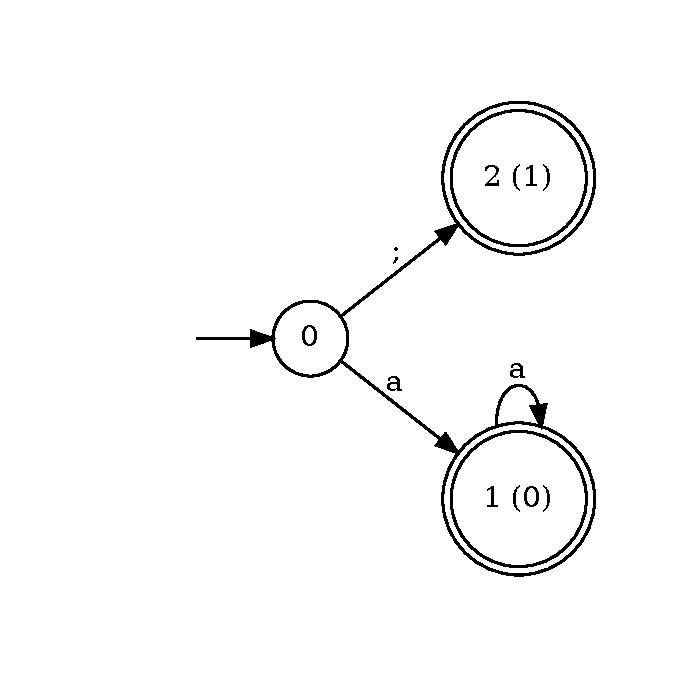
\includegraphics[width=\linewidth]{figures/certificate_sound.pdf}\\[0.5em]
(a) $a^+$ and \code{;}
\end{minipage}
\hfill
\begin{minipage}[b]{0.24\linewidth}
\centering
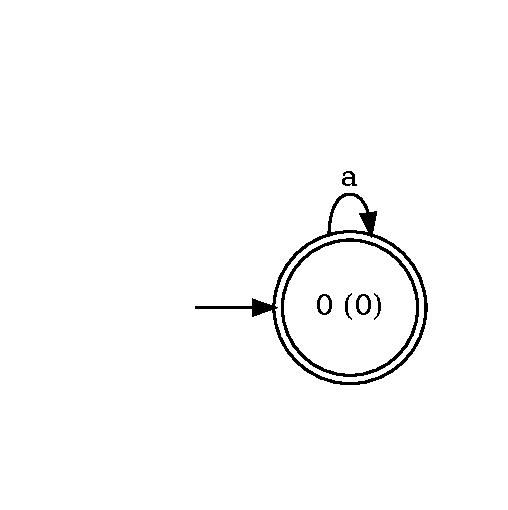
\includegraphics[width=\linewidth]{figures/certificate_nullable.pdf}\\[0.5em]
(b) $a^*$
\end{minipage}
\hfill
\begin{minipage}[b]{0.3\linewidth}
\centering
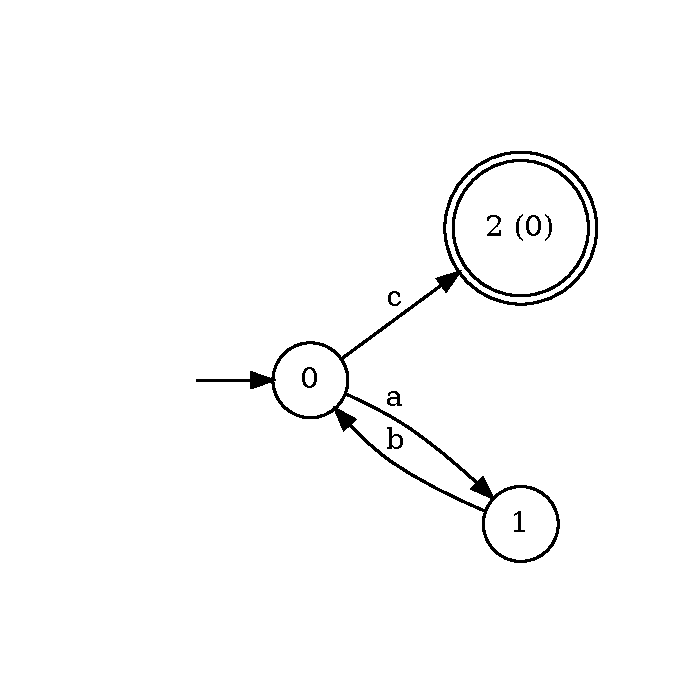
\includegraphics[width=\linewidth]{figures/certificate_cyclic.pdf}\\[0.5em]
(c) $(ab)^*c$
\end{minipage}
\caption{Minimized automata drawn by the library described here; double circles are accepting states,
labelled with the state number and the token identifier. In (a) nothing enters state 0, so \code{;} is certified: no
other state consumes it. In (b) state 0 accepts and re-enters itself on $a$, and in (c) it is re-entered through the
cycle $a, b$. In both counterexamples the only state consuming the candidate byte is the initial one, so dropping the
re-entrancy condition would certify it and break longest match. The shipped predicate rejects the candidate in (b) and
(c) and accepts \code{;} in (a).}
\label{fig:reentrancy}
\end{figure}

\section{Certification modulo discarded tokens}
\label{sec:modulo}

Fix a set $I \subseteq T$ of \emph{discarded} tokens, chosen by the caller. Write $\pi_I$ for the map on token sequences
deleting every pair whose token lies in $I$, and call two sequences \emph{$I$-equivalent} when $\pi_I$ sends them to the
same sequence. Comparing streams modulo a designated token class is not itself new: ZipLex's separator construction
proves its printing guarantee in exactly this form, re-lexing equal up to inserted separator
tokens~\cite{chassot2026ziplex}. What is asked here is different: which symbols of raw input may be cut at while
preserving $I$-equivalence, where the cut can land inside an existing discarded token rather than at a seam between
formed tokens.

Being discarded is not by itself sufficient. Cutting the line comment \code{//ab} between its last two bytes leaves
\code{//a} on the left, which is a comment and is discarded, and \code{b} on the right, which is an identifier and is
not. What is required is that both halves of the severed token are discarded, and that the restarted scan rejoins the
scan it interrupted. Write
\[
T(q) = \{\, \tau(p) \mid p = (\delta^+)^*(q, v) \text{ for some } v \in \Sigma^*,\ \tau(p) \text{ defined} \,\}
\]
for the tokens still reachable from $q$, noting $\tau(q) \in T(q)$ whenever $\tau(q)$ is defined.

\begin{definition}[Certified modulo $I$]
\label{def:trivia-certified}
A symbol $b \in \Sigma$ is \emph{certified modulo $I$} if every $q \in Q^+$ with $\delta^+(q, b)$ defined satisfies
$A(q)$ or $C(q)$, where
\[
A(q) \;\equiv\; q = q_0 \text{ and } q_0 \text{ is not re-entrant},
\]
and $C(q)$ holds when all three of
\begin{enumerate}
  \item $\tau(q)$ is defined,
  \item $\delta^+(q_0, b)$ is defined and equal to $\delta^+(q, b)$, and
  \item $T(q) \subseteq I$
\end{enumerate}
are satisfied.
\end{definition}

The two alternatives are not symmetric, and the asymmetry matters. $A(q)$ is Definition~\ref{def:certified}: the
initial state may consume $b$ only while nothing returns to it mid-scan. $C(q)$ is the relaxation, and it is available
to \emph{every} consuming state including a re-entered $q_0$. Requiring $A$ of $q_0$ unconditionally would be strictly
weaker than necessary: for a discarded token \code{a*} the minimized automaton is one accepting, self-looping state,
so $q_0$ is re-entrant and $A$ fails, yet $C(q_0)$ holds and cutting between two \code{a}s replaces one discarded
token by two, which $\pi_I$ deletes either way.

Setting $I = \emptyset$ recovers Definition~\ref{def:certified} exactly, since $\tau(q) \in T(q)$ makes clause 3
unsatisfiable and only $A$ survives; so every certified symbol is certified modulo $I$ for every $I$. The three
conditions of $C$ do distinct work. That $\tau(q)$ is defined lets the left chunk stop at the cut with a complete token
rather than mid-token. That $T(q) \subseteq I$ makes that token and whatever the severed remainder becomes both
discardable, and since $\tau(q) \in T(q)$ it also forces the left chunk's token to be discarded. The equality
$\delta^+(q, b) = \delta^+(q_0, b)$ is the load-bearing condition: after consuming $b$ the restarted scan occupies the
same state as the scan it interrupted, so the two agree on every subsequent byte and the disturbance is confined to the
single token containing the cut. Without it the definition would be a statement about language inclusion rather than a
test on the transition table. Such a statement may still be decidable, but deciding it would need a construction over an
augmented scanner semantics, one carrying lookahead and token output as state composition for maximal munch must, rather
than the comparison of two table rows used here.

\begin{theorem}[Split invariance modulo $I$]
\label{thm:trivia}
Let $w$ be completely tokenizable and let $0 = c_0 < c_1 < \cdots < c_m = |w|$ be offsets such that each interior
$c_j$ holds a symbol certified modulo $I$. Then
\[
\pi_I(\mathrm{tok}(w)) \;=\; \pi_I\!\left(\mathrm{tok}(w_{[c_0,c_1)}) \cdot \mathrm{tok}(w_{[c_1,c_2)}) \cdots
\mathrm{tok}(w_{[c_{m-1},c_m)})\right),
\]
where $\cdot$ denotes concatenation of token sequences and $w_{[a,b)}$ the corresponding slice.
\end{theorem}

\begin{proof} For empty $w$ the partition degenerates as in Theorem~\ref{thm:main} and both images are empty; assume
$|w| > 0$. By induction on $m$ it suffices to treat one interior cut at $c$ holding $b$. The induction is well founded
because the one-cut argument below shows each chunk consumes its whole slice, so both slices are themselves completely
tokenizable and the remaining cuts may be applied to them in turn.

Suppose first that $c$ is a token boundary of $w$. The left slice $w_{[0,c)}$ emits the same tokens as $w$ on $[0,c)$
by Lemma~\ref{lem:truncation} taken with $s = c$, which is what rules out a last token whose failed lookahead crossed
$c$ in $w$. The scanner enters every token in $q_0$ and carries no state across boundaries, so the chunk beginning at
$c$ starts in the same state as the scan of $w$ does there and reads the same bytes. The token sequences on the two
sides are therefore equal before $\pi_I$ is applied, and $\pi_I$ preserves equality.

Otherwise $c$ lies strictly inside an emitted token spanning $[s, e)$ and carrying token $t$. Let $u = w_s \cdots
w_{c-1}$, which is nonempty, and let $q = (\delta^+)^*(q_0, u)$ be the state immediately before $b$ is consumed. The
token's match path continues through $c$, so $\delta^+(q, b)$ is defined and $q$ satisfies $A(q)$ or $C(q)$. It cannot
satisfy $A(q)$: that would need $q = q_0$ with $q_0$ not re-entrant, yet $(\delta^+)^*(q_0, u) = q_0$ with $u$
nonempty is precisely re-entrancy. So $C(q)$ holds, and it holds whether or not $q$ happens to be a re-entered $q_0$;
that is the only place the generalization over Definition~\ref{def:certified} is used.

Consider the chunk ending at $c$, which is the prefix $w_{[0,c)}$ with $c > s$. By Lemma~\ref{lem:truncation} it emits
the same tokens as $w$ on $[0, s)$ and reaches $s$ in $q_0$; that is what rules out an earlier token whose failed
lookahead ran past $s$ in $w$ and is truncated here. The chunk then consumes $u$ and arrives at $q$ with the chunk
exhausted. Since $\tau(q)$ is defined by condition 1, the last accepting position recorded is $c$ itself, so the chunk
emits the single token $\tau(q)$ spanning $[s, c)$ and consumes to its end.

Consider the chunk beginning at $c$. It starts in $q_0$ and consumes $b$, reaching $\delta^+(q_0, b)$, which equals
$\delta^+(q, b)$ by condition 2, the state the scan of $w$ occupies after consuming the same byte at the same offset.
From there both runs read identical bytes from identical states, so they record identical accepting positions, and the
chunk emits $t$ spanning $[c, e)$. Both runs then stand at $e$ in $q_0$, and $e$ is a boundary of $w$, so the
remainders agree.

The two sides therefore differ only in that $t$ on $[s, e)$ is replaced by $\tau(q)$ on $[s, c)$ followed by $t$ on
$[c, e)$. Both $\tau(q)$ and $t$ lie in $T(q)$, which condition 3 places inside $I$, so $\pi_I$ deletes all three
occurrences and the images coincide.
\end{proof}

Corollary~\ref{cor:malformed} has no analogue here. For input the serial scan does not tokenize completely, no
$\pi_I$-prefix relation is claimed, and a caller must still check every chunk's consumed length before trusting the
concatenation at all.

\begin{proposition}[Useful certificates modulo $I$]
\label{prop:useful}
Proposition~\ref{prop:vacuous} and Corollary~\ref{cor:useful} carry over: a symbol no live state consumes is certified
modulo $I$ for every $I$ and occurs in no completely tokenizable input, and a symbol certified modulo $I$ is
non-vacuous exactly when $\delta^+(q_0, b)$ is defined.
\end{proposition}

\begin{proof}
The first two claims are those of Proposition~\ref{prop:vacuous}, whose argument does not depend on which of the two
conditions admitted $b$: Definition~\ref{def:trivia-certified} likewise quantifies over an empty set. For the third,
every state consuming $b$ live satisfies $A$, hence is $q_0$, or satisfies $C$, whose clause 2 gives $\delta^+(q, b) =
\delta^+(q_0, b)$; either way some live state consumes $b$ exactly when $\delta^+(q_0, b)$ is defined.
\end{proof}

As in the exact setting, such symbols are certified but useless: a caller cannot act on one, and a planner searching
for one scans the whole input for nothing. Both the library predicate and every table below therefore report the
\emph{useful} set, intersecting the certificate with the initial state's live transitions. This matters for reading
Table~\ref{tab:applicability}: the JSON row omits the raw control bytes that no token admits, which the definitions
certify vacuously, and reports only the bytes an input can actually contain.

\begin{proposition}[Strict extension]
\label{prop:extends}
Every certified symbol is certified modulo $I$ for every $I \subseteq T$, and there are token sets and sets $I$ for
which the converse fails.
\end{proposition}

\begin{proof}
The first claim is immediate, since Definition~\ref{def:trivia-certified} offers $q = q_0$ as an alternative and its
re-entrancy proviso is that of Definition~\ref{def:certified}. For the second, take identifiers, punctuation and a
whitespace run over space and newline, with the whitespace token in $I$. Newline is not certified, since the state
inside a whitespace run consumes it into a co-accessible state; it is certified modulo $I$, since that state accepts
the whitespace token, reaches no other token, and advancing from it and from $q_0$ on newline both reach the run
state.
\end{proof}

\section{Deriving and using the certificate}
\label{sec:derivation}

The certificate is derived by a linear-time analysis of the compiled transition table at construction time. First a
reverse pass computes co-accessibility: the table is inverted into a predecessor list, the accepting states seed a
worklist, and each state that reaches one is marked. A forward pass from $q_0$ then marks the reachable states, and
intersecting the two marks yields $Q^+$, the trim subautomaton the results are stated over; subset construction emits
only reachable states, but the analysis is exposed on a simulator that accepts any transition table, and an unreachable
state left by a hand-assembled one would otherwise produce false negatives. One scan then detects whether any reachable
entry targets $q_0$, establishing re-entrancy, and a sweep over the $|\Sigma| \times |Q|$ table records, for each byte,
whether any non-exempt reachable live state consumes it into $Q^+$. The result is a $|\Sigma|$-bit set. Every pass
visits each entry of the logical $|\Sigma| \times |Q|$ table a constant number of times, rereading a shared class
row where the physical table is class-compressed, so the cost stays $O(|Q|\,|\Sigma|)$, with the same bound in
auxiliary space for the predecessor list; it is paid once, at the same asymptotic order as building the table itself,
and the scanner's inner loop is untouched.

Three operations expose the property. A predicate reports whether a byte is a useful certified split symbol, the set
of Corollary~\ref{cor:useful}. A planner divides an input into chunks by sliding each interior boundary forward from
its equal-division target to the next certified byte, and returns a single chunk spanning the whole input when that
useful set is empty. An executor runs the plan, one thread per chunk, and by Theorem~\ref{thm:main} the concatenated
per-chunk streams equal the serial stream for completely tokenizable input, with Corollary~\ref{cor:malformed}
governing the rest. There is no speculation to retry, no overlap to verify, and no merge beyond concatenation.

For $k$ requested chunks the planner performs at most $k-1$ forward searches, so its worst case is $O(kN)$ over an
input of $N$ bytes when certified occurrences are rare; $k$ is normally a small hardware-thread count, and the
searches start at equally spaced offsets. A one-pass planner would reduce the worst case to $O(N + k)$.
Section~\ref{sec:planning} measures the range.

\begin{figure}[t]
\centering
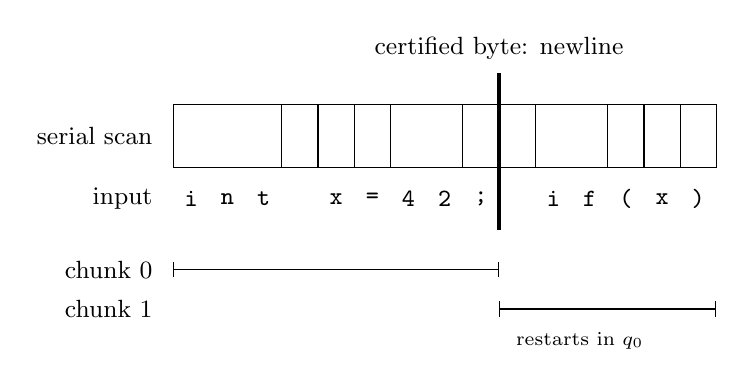
\begin{tikzpicture}[x=4.6mm, y=1mm, font=\small]
  % One cell per input byte, so the token boxes and the input line up exactly.
  % i n t _ x = 4 2 ; \n i f ( x )
  %  0 1 2 3 4 5 6 7 8  9 10 11 12 13 14
  \node[anchor=east] at (-0.3, 13) {serial scan};
  \node[anchor=east] at (-0.3, 5) {input};

  % token extents, as outlined boxes
  \foreach \s/\e in {0/2, 3/3, 4/4, 5/5, 6/7, 8/8, 9/9, 10/11, 12/12, 13/13, 14/14} {
    \draw (\s, 9) rectangle (\e + 1, 17);
  }

  % the input bytes, one per cell
  \foreach \i/\c in {0/i, 1/n, 2/t, 4/x, 5/=, 6/4, 7/2, 8/;, 10/i, 11/f, 12/(, 13/x, 14/)} {
    \node at (\i + 0.5, 5) {\ttfamily \c};
  }

  % the certified byte, and the boundary immediately before it
  \draw[very thick] (9, 1) -- (9, 21);
  \node[anchor=south] at (9, 21.5) {certified byte: newline};
  % the two chunks
  \node[anchor=east] at (-0.3, -4) {chunk 0};
  \draw[|-|] (0, -4) -- (9, -4);
  \node[anchor=east] at (-0.3, -9) {chunk 1};
  \draw[|-|] (9, -9) -- (15, -9);
  \node[anchor=west] at (9.2, -13) {\scriptsize restarts in $q_0$};
\end{tikzpicture}
\caption{A certified byte is a point where the serial scan is provably between tokens: no state reachable mid-token
consumes it into a state that can still accept, so the scan has finished its last token by that offset and restarts
there in $q_0$; failed lookahead may have read past the offset, but recorded no acceptance beyond it. A chunk may
therefore start at that offset with no entry-state uncertainty, and the two chunks' token streams concatenate to the
serial one.}
\label{fig:split}
\end{figure}

\subsection{Deciding the relaxed condition}
\label{sec:decide}

Condition 3 needs no per-state set of tokens. Because $I$ is fixed when the automaton is compiled, $T(q) \subseteq I$
is the complement of ``some kept token is still reachable from $q$'', which one reverse search settles for every state
at once: seed it with the accepting states whose token lies outside $I$ and close backwards along transitions, then
$T(q) \subseteq I$ exactly when $q$ was not reached. Two details keep that linear. The closure walks a reverse index
of the transition table rather than rescanning every symbol and source state for each state it reaches, which would be
quadratic in the state count; and whether a state accepts a discarded token is resolved once per state rather than
searched for from inside the symbol loop. The index needs no space of its own, since determining co-accessibility
already builds one and the relaxed analysis reuses it; it is built once per class row rather than once per symbol
value, so it stays the order of the class-compressed table actually stored rather than of an uncompressed $|Q| \times
|\Sigma|$ one. The closure then costs $O(|Q| + E)$, where $E$ counts the stored table edges, and the per-symbol test
that follows costs $O(|Q|\,|\Sigma|)$. The implementation holds the discarded set in an ordered set, so constructing
it costs $O(|I| \log(1 + |I|))$ and resolving one state's membership $O(\log(1 + |I|))$, for
$O(|Q|\,|\Sigma| + (|Q| + |I|) \log(1 + |I|))$ overall in $O(|Q| + |I|)$ additional space, excluding the predecessor
index the exact analysis already builds and this one reuses.
Propagating the sets $T(q)$ themselves would instead need $O(|Q|\,|T|)$ storage. Testing one symbol then walks the
states as the exact condition does, adding a membership test and one lookup of $\delta^+(q_0, b)$ that is constant
across the walk. The outcome packs into a second 256-bit map, held beside the exact one, so the run-time predicate
remains a single bit test and the search for a chunk boundary is unchanged. The relaxation is therefore free at scan
time. At build time it is additional work rather than a substitute: a backward closure over a reverse index that is
built either way, one membership test per state, and a second sweep of the same $|Q|\,|\Sigma|$ shape as the exact
one, which runs whether or not a caller ever asks the weaker question.

One consequence constrains the interface rather than the theory. The map depends on $I$, so a lexer must be told which
tokens the caller discards when it is built rather than being asked at each call. In practice the discarded set is
fixed by the consuming tool when the lexer is built and does not vary with the input, so this is a mild restriction,
but the relaxed certificate is not a drop-in query on an existing lexer, and two consumers of one grammar that
discard different tokens, a compiler and a formatter say, hold different certificates.

The condition is sound and conservative rather than exact. We tested both directions against an exhaustive oracle:
over 400 randomly generated token sets on a three-symbol alphabet, every string up to length eight was tokenized,
split at every occurrence of every symbol, and the $\pi_I$ images of the spliced and serial streams compared. Of the
symbol and token set pairs the corpus exercised, 265 were admitted by Definition~\ref{def:trivia-certified} and none
of them failed, and no symbol admitted by Definition~\ref{def:certified} was ever lost, which is
Proposition~\ref{prop:extends} checked mechanically. A further 97 pairs had no counterexample through length eight yet
were rejected, so close to one such pair in four is refused. Those 97 are only pairs for which no counterexample
exists through length eight, so they do not by themselves establish conservatism; raising the bound from six to eight
reclassified two of them, which shows the count is bound-sensitive rather than settled. What does establish
conservatism is the explicit witness below. These counts describe one generator and are stated only because
\code{validation.cpp} in the artifact reproduces them exactly; they are seeded and their draw order is pinned, so they
do not vary between compilers.

A proportion from a random sweep describes the generator as much as the condition, so it is worth naming a witness.
Take the discarded tokens \code{ab*} and \code{b+} alongside a kept token \code{c}, over a letter neither uses.
Splitting at a \code{b} inside an \code{ab*} token is always safe modulo the discarded kinds, since the left piece is
a shorter \code{ab*} and the right is a \code{b+}, both discarded. The only other home a \code{b} has is inside a
\code{b+} token, where the cut leaves two shorter \code{b+} pieces, discarded as well, so every occurrence of \code{b}
is safe. Condition 2 nonetheless fails: advancing on \code{b} from inside \code{ab*} reaches a state accepting
\code{ab*}, advancing on \code{b} from the initial state reaches one accepting \code{b+}, and since those accept
different tokens minimization keeps them apart. Insisting that the two scans reconverge at once is what makes the test
local, and this is what it costs: the equality is necessary for this local certificate, not for semantic safety, which
the witness retains without it. The sweep figures and this witness are both asserted by \code{validation.cpp} in the
artifact. Because the automaton is minimized before the test, the state equality in condition 2 is as tight as the
minimizer of Section~\ref{sec:necessity} makes it, which is tighter than no minimization and weaker than
Myhill-Nerode, since that minimizer keeps empty-right-language states apart. It is not the tightest conceivable test:
a quotient treating accepting labels in $I$ as observationally equivalent could merge states this one keeps apart, and
the witness above is exactly such a pair. Both directions are additionally carried as property tests over randomly
generated automata in the munch lexer library~\cite{munch}. Those are a separate and independently parameterised
sweep, over a four-symbol alphabet to a shorter bound. Both sweeps query the shipped predicate rather than a private
copy of the rule, which is deliberate: a test of a reimplementation would justify the reimplementation. What is
independent between them is the generator and the oracle, so their agreement is evidence that the predicate meets the
specification on two unrelated families of automata, not that two codings of the rule agree.

\section{Applicability}
\label{sec:applicability}

The certificate asks the grammar for cooperation, and the interesting question is how much real token sets give.
Table~\ref{tab:applicability} was produced by compiling each token set and reading the predicate for all 256 byte
values. The predicate implements Corollary~\ref{cor:useful}, so it excludes the vacuous certificates of
Proposition~\ref{prop:vacuous} already and the column needs no further filtering. Rows two through four each add a
single token kind to the grammar of row one rather than accumulating, so each collapse is attributable to the token
kind named; the conventional and split-friendly rows recognize exactly the same byte language and differ only in the
tokenization, and the block-comment row directly after them adds one token kind to the split-friendly grammar, so
those three are read together. The program that produces the table is \code{figures/applicability.cpp}, archived with
this report; it links the library and asserts every row.

\begin{table}[t] \centering \begin{tabular}{p{7.0cm}p{3.6cm}p{3.6cm}} \toprule Token set & Useful certified & Useful
modulo $I$ \\ \midrule C-like: identifiers, numbers, whitespace runs, operators, punctuation & all operator and
punctuation bytes & the same, plus space, tab and newline \\ the first row plus string literals alone (no raw newline
inside) & none & newline \\ the first row plus \code{//} line comments alone & none & newline \\ the first row plus
block comments alone & none & the same \\ JSON, the RFC 8259 lexical forms over bytes & none & tab, newline, carriage
return \\ log lines: a run of non-newline bytes, and newline & newline & the same \\ C-like, conventional
tokenization: line-bounded strings and \code{//} comments, whitespace runs including newline & none & newline \\ the
same recognized language, split-friendly: newline its own token, spaces and tabs a separate run & newline & the same
\\ the same plus block comments & none & the same \\ \code{keyword\_scale\_builder()}, the construction-cost grammar &
16 of those 24 bytes & the same, plus space, tab and newline \\ \code{build\_lexer(false)}, the scaling grammar & 13
of its own 14 & the same, plus space, tab and newline \\
\bottomrule
\end{tabular}
\caption{Certified bytes by token
set, exactly and modulo the discarded set $I$. Three mechanisms explain the collapses in the middle column:
free-content tokens absorb the alphabet, run tokens de-certify their own bytes, and a multi-byte token de-certifies
the bytes it continues past. Discarding undoes exactly one of them, the second: a severed whitespace run leaves two
whitespace runs and both are deleted, so the run-token obstruction alone is removed; a string, comment or kept token
that also admits the byte still excludes it. The other two survive it: a state inside a string literal or a block
comment accepts nothing, so no cut there ends the left chunk on a complete discarded token, and a kept multi-byte
token keeps its continuation bytes lost, since the token such a cut severs is kept and cannot vanish from the streams.
Both columns are asserted for every row by \code{figures/applicability.cpp}; the exact column is the shipped
predicate, and the relaxed column is the same predicate given the row's discarded set, with four rows additionally
confirmed by splitting a corpus.}
\label{tab:applicability}
\end{table}

Three mechanisms explain the collapses. First, \emph{free-content tokens absorb the alphabet}: a string literal that
may contain \code{(} makes \code{(} a mid-token byte and de-certifies it everywhere, so one token kind with a
near-total interior alphabet removes almost every candidate. Second, \emph{run tokens de-certify their own bytes}:
with whitespace tokenized as a run over space, tab, and newline, the second newline of a blank line is consumed by the
run's continuation state, so newline itself becomes mid-token-consumable. The byte's own token kills it, which is easy
to miss.

Third, and in the same family, \emph{a multi-byte token de-certifies every byte that can follow its first}. The
study's first row spells each operator as a single byte, so each is consumed only at the initial state and all
twenty-four certify. Section~\ref{sec:evaluation} measures two different C-like grammars, and the last two rows of
Table~\ref{tab:applicability} name them rather than describing them, since they disagree. The construction-cost
grammar, \code{keyword\_scale\_builder()} in \code{tools/benchmark/src/main.cpp}, spells operators as literals
including \code{++}, \code{==} and \code{->} and admits a decimal point inside a number. Every byte occurring after
the first position of some operator therefore has a live mid-token state on it, and seven candidates fall that way:
\code{= < > \& | + -}. The decimal point falls independently, not as an operator continuation but because
\code{decimal\_float()} admits it inside a number, bringing the total to eight. The scaling grammar,
\code{build\_lexer(false)} in \code{tools/benchmark/src/harness.cpp}, has a smaller operator set in which every
multi-byte operator has \code{=} as its only continuation byte, so only \code{=} is lost and thirteen of its fourteen
candidates certify. Both collapses are partial. What they show is that ``operators certify'' is a claim about the
particular literals a grammar registers, so the grammar has to be named rather than described: these two C-like
benchmark grammars recognize different operator and number languages, and they certify different sets. The sharper
claim, that certification depends on the tokenization and not on the recognized language, needs a pair recognizing the
same language, and the conventional and split-friendly rows below are that pair: identical accepted input, differing
only in whether newline is folded into the whitespace run or carries a kind of its own, and certifying nothing versus
certifying newline. The kinds therefore differ by exactly that one token, which is the change under study.

All three mechanisms point at the same design lever: certification is a property of the \emph{tokenization} rather
than an intrinsic one, and a tokenization can sometimes be refactored without changing what is recognized at all. The
split-friendly row of Table~\ref{tab:applicability} keeps the identical C-like language but tokenizes newline as its
own single-byte token, leaves spaces and tabs as whitespace runs, and keeps strings and line comments line-bounded.
The row directly above it is the same language under the conventional tokenization and certifies nothing, which
isolates the change. Then newline certifies, and the folklore rule follows as a practical corollary: for tokenizations
in which newline is its own token, line-based splitting is sound when no other token can contain a newline. The
automaton-level statement remains the exact one; ``no token spans a line'' is sufficient here but not necessary in
general, since a token that merely \emph{begins} with newline leaves the certificate intact. Adding block comments,
the one token kind in the split-friendly tokenization studied here that spans lines, destroys the certificate again,
which is the formal shape of both ``you cannot chunk C by lines'' and the quoted-newline problem that pushed CSV
parsing into speculation.

The JSON row of Table~\ref{tab:applicability} appears to contradict the literature, and the reconciliation is about
the equivalence each result preserves rather than about the automaton. Prior claims that JSON may be divided at
newline~\cite{barenghi2015parallel,li2021plex} rest on a weaker one. Barenghi et al.'s sequential lexing algorithm
appends a byte to the lexeme buffer only when it is not reading a whitespace character outside a string or a comment,
so whitespace is unobservable in its output; Plex restates the claim on the different ground that newline occurs in no
lexeme, which holds only once whitespace runs are not themselves counted as lexemes. Either way the division can split
one maximal whitespace match into two discarded matches whose lengths sum to the original, leaving the surviving
stream unchanged. Theorem~\ref{thm:main} preserves something stronger, the complete sequence of emitted kinds and
lengths, and under that semantics a newline inside a maximal whitespace token is not a certified boundary. The grammar
studied here follows the RFC 8259 lexical forms~\cite{bray2017json} over byte input, with the full string escapes,
signed numbers with fraction and exponent, the three literal names, and whitespace runs emitted as tokens, so it is
refused exactly as it should be. It is a lexer over bytes rather than a conforming JSON processor: string interiors
admit any byte from \code{0x20} up except quote and backslash, so UTF-8 well-formedness, which RFC 8259 requires of
JSON exchanged outside a closed ecosystem, is assumed of the input rather than checked here. That is orthogonal to
certification, since validating it would only remove bytes from string interiors and so could not de-certify anything
that certifies now. The two results do not conflict; they quantify over different streams, and this paper supplies
both. Definition~\ref{def:certified} rejects newline for JSON, since the whitespace continuation state consumes it
either way, and Theorem~\ref{thm:trivia} accepts it once whitespace is declared discarded: that is precisely the JSON
row of Table~\ref{tab:applicability}, none exactly and tab, newline and carriage return modulo $I$. The prior claim is
therefore not merely reconciled but derived, from the token set rather than from a reading of the format. Recovering
certification under the \emph{exact} equivalence still needs the tokenization changed, by making newline its own token
as the split-friendly row does.

The right column of Table~\ref{tab:applicability} places the whitespace and comment tokens of each row in $I$ and
reads the relaxed condition. Seven of the eleven rows gain bytes, and the pattern behind them is the second of the
three collapse mechanisms named above: wherever whitespace is a run token the caller discards, its own bytes come
back, because severing a whitespace run at a whitespace byte yields two whitespace runs and both are deleted. That is
the one mechanism discarding undoes. The other two survive it. A byte a string literal or a block comment absorbs is
recovered nowhere: a state inside either accepts nothing at all, so the left chunk cannot end there on a complete
discarded token, which is the first thing $C$ requires. A byte a kept multi-byte token continues past is likewise not
recovered: the state that has consumed its first byte can still reach the kept token, so the third clause of $C$
fails, and rightly, since severing a kept token is a difference the deletion preserves.

In the exact column each outcome reports a fact about the tokenization rather than a limitation of the test, since
Theorem~\ref{thm:necessity} makes that condition necessary as well as sufficient. The modulo column carries no such
licence: it is conservative, so a byte absent there may still be safe modulo $I$ and merely refused, and only its
positive entries are statements about the pair of token set and discarded set. Newline is recovered for the
conventional C-like token set because line-bounded strings and \code{//} comments cannot contain one, so a whitespace
run is the only token whose interior admits it. Space is recovered in no C-like row carrying strings or comments,
since it sits legally inside both; the first row, which has neither, recovers it along with tab and newline. The JSON
row is the same lexer over bytes, its UTF-8 caveat unchanged from above. JSON gains tab and carriage return as well as
newline because RFC 8259 excludes every raw byte below \code{0x20} from string interiors, which confines all three to
whitespace, while space is admitted there and so is not recovered. That the recovered set is exactly JSON's whitespace
minus space is a consequence of the RFC's own exclusion, not a coincidence. The rows carrying block comments continue
to certify nothing, because a comment severed at a newline leaves \code{/*\,a} and \code{b\,*/}, and both halves
re-tokenize completely: in this token set they become the operators \code{/} and \code{*} and an identifier, six kept
tokens in place of one discarded comment, which is exactly the difference a caller can see. The correct conclusion is
that this tokenization of a C-like language with block comments cannot be split before every newline without state,
overlap, speculation or repair, and the certificate says so.

Four rows are cross-checked by splitting as well as by reading the predicate: the conventional and split-friendly
C-like pair, the split-friendly row with block comments, and JSON. On those the condition agrees with brute-force
splitting on every candidate byte the corpus exercises, which is a declared set of sixteen bytes, the whitespace kinds
plus eleven representative structural characters, not all 256. The conservatism measured in Section~\ref{sec:decide}
therefore did not appear on the bytes tested, which is weaker than exactness on those token sets and is all the
artifact checks.

The practical content is narrower than a count of moved cells suggests, and more useful. The exact certificate already
admitted newline for the split-friendly tokenization in which newline is its own token and whitespace runs exclude it.
That is a redesign of the token set imposed on the user by the parallelization technique. Theorem~\ref{thm:trivia}
removes the imposition: the conventional whitespace rule that hand-written lexers already contain certifies newline
without modification, so the conventional and split-friendly rows give the same answer and the redesign buys nothing
for a caller comparing streams modulo $I$. The relaxation is better read as widening the class of token sets the
method accepts as written than as adding split points to a fixed one.

\subsection{Framing at the producer}
\label{sec:framing}

Definitions~\ref{def:certified} and~\ref{def:trivia-certified} quantify over the automaton, the second also over the
declared discarded set, and mention no input. Certification is therefore static, in the token set alone for the exact
condition and in the pair of token set and $I$ for the relaxed one, and no transformation applied when reading a
document
can make a byte certified that was not. This rules out an appealing idea directly: one cannot normalize input at read
time to manufacture split points. It also explains why the obvious attempt is circular, since deciding which
occurrences of a byte lie inside a token is the sequential problem that chunking was meant to avoid.

What can be arranged is a guarantee about a particular document, supplied by whatever produced it. Reserve a byte that
no token admits in its interior, give it a rule of its own, and require the producer to emit it only at token
boundaries and to escape it wherever it would otherwise appear inside a token. The reserved byte's only live
consumption is then from $q_0$, and Definition~\ref{def:certified} admits it outright with no appeal to
Theorem~\ref{thm:trivia}.
Applied to the block-comment row of Table~\ref{tab:applicability}, whose certified set is empty under both conditions,
reserving \code{0x1E} yields a certified split symbol, and a framed document splits at every occurrence with the token
stream reproduced exactly, including across block comments spanning lines and string literals containing punctuation.

None of that construction is new. ASCII reserves \code{0x1E} as \textsc{record separator}, one of four information
separators defined for exactly this kind of framing~\cite{cerf1969ascii}, JSON text sequences standardize precisely that
byte as a record prefix~\cite{williams2015rfc7464}, and informal newline-delimited JSON makes the same bargain in
different notation without the reserved byte, while length-prefixed framing and columnar row groups buy random access by
other means and are analogies rather than instances; Barenghi et al.~\cite{barenghi2015parallel} reach a comparable
place by constraining the source language instead. Chassot and Kun{\v{c}}ak~\cite{chassot2026ziplex} study a different
but closely related maximal-munch boundary question for invertible lexing. Given already formed adjacent tokens, their
sound R-Path relation checks whether the first token's text followed by the next token's first symbol remains a prefix
of any rule; their separator construction can instead insert a separator during printing and compare the re-lexed stream
modulo separator tokens. These operations protect known token sequences during printing and recombination; they neither
locate cuts in raw input nor derive bytes safe at every occurrence before lexing. What the certificate contributes is
the check. A format designer choosing a delimiter is making a claim about every token the grammar admits, and
Definition~\ref{def:certified} decides that claim from the compiled automaton rather than leaving it to inspection. Read
this way an applicability table is not only a report of where the method applies but a design rule for formats intended
to be chunked. A row whose exact column is empty is a warning, by Theorem~\ref{thm:necessity}, that no single-byte
delimiter preserves the exact stream without changing the token set; an empty modulo column is only a refusal, since
that condition is conservative.

The limit is equally clear. A document already written cannot be reframed without reading it, so this recovers nothing
for a compiler consuming source it did not generate. It applies where the writer cooperates, which covers generated
code, logs, exports and interchange formats, and not to arbitrary input.

\section{Evaluation}
\label{sec:evaluation}

The evaluation reports two machines. The first is the one the method was developed on and is retained because the
contrast with the second is itself a result: a figure that looks like a property of the API on one does not hold its
value, or even its sign, across environments and benchmark revisions.

Everything measured here uses the exact certificate. Both \code{chunk\_boundaries()} and the parallel executor built on
it consult the exact map, so no figure in this section reports what the relaxed condition would buy at run time.
Section~\ref{sec:applicability} establishes which bytes it recovers, and that is a statement about token sets rather
than about throughput; a token set that certifies nothing exactly can gain a boundary set from the relaxation, as seven
of the eleven rows studied do and the block-comment rows do not, but turning that into a measured speedup needs a
planner this library does not yet ship.

\paragraph{Environment A, virtualized.} An Intel Core i9-12900K, a hybrid part with eight performance cores carrying
two-way SMT and eight efficiency cores, so sixteen physical cores and 24 logical processors, with 32\,GiB of memory.
The host is Windows 11 build 26200 with virtualization-based security enabled; the measurements ran under WSL 2.7.11
on kernel 6.18.33.2-microsoft-standard-WSL2, Ubuntu 24.04.4 LTS, glibc 2.39, with all 24 logical processors and
15\,GiB of memory visible to the guest. Compiled by GCC 13.3.0 at \code{-O2}. Corpora are 16\,MiB and fixed-seed,
scenarios run in a fixed order, and the archive holds summaries only (\code{data/benchmark.txt}), whose header
records the machine, operating system, compiler and command; the Windows build, WSL and kernel versions, memory and
topology details above are author-recorded rather than archived.

Four properties of this environment bound what its figures establish, and we state them rather than adjust for them. The
guest does not see the host's hybrid topology: it reports twelve cores of two threads each, so a performance core is
indistinguishable from an efficiency core from inside the measurement. Threads are not pinned, and could not usefully be
while that holds. The guest is given no \code{cpufreq} interface, so the clock is neither fixed nor observable. And the
machine was not quiesced. The corpora also fit in cache, 16\,MiB against a 30\,MB last-level cache, so the run targets
warm-cache conditions rather than certifying residency throughout.

\paragraph{Environment B, bare metal.} An AMD Ryzen 9 9950X3D, sixteen physical cores with two-way SMT across two L3
domains of eight cores each, 128\,MiB of L3 in total, 59\,GiB of memory, Ubuntu 26.04 on kernel 7.0.0-28-generic,
compiled by GCC 15.2.0 at \code{-O2}. The \code{performance} governor was set, which biases the clock toward its maximum
but does not fix it: boost remains enabled, and the archived \code{lscpu -e} of the pinned run reported in
Table~\ref{tab:scaling} shows 22 distinct frequencies between 624 and 5711\,MHz across the 32 processors at the instant
it was taken. The clock is therefore observable here, unlike in Environment A, but not controlled. The topology is
visible and archived; the ten scaling scenarios run in interleaved rounds reshuffled per round from a fixed seed, while
the construction, planning and thread-launch scenarios run as blocks; and corpora sweep 1, 16, 128 and 512\,MiB in that
fixed ascending order. Every pass of the ten scaling scenarios is recorded individually in
\code{data/bare-metal-unpinned-run2/} and \code{data/bare-metal-pinned-run2/}; the construction, planning and
thread-launch figures below are summaries over 15 passes, not per-pass records.

This environment is measured in two placements, each run twice, giving four archives. The unpinned runs may place
threads on any of the 32 logical processors. The pinned run confines the process to the eight physical cores of a
single L3 domain (\code{taskset -c 0-7}), which excludes the SMT siblings and the other L3 domain from the set the
scheduler may use, so eight threads have eight distinct physical cores available to them. The archives certify the
width of that mask but not its members: the collector recorded \code{nproc} as 8 from inside the affinity mask, while
the archived \code{lscpu -e} describes the whole machine, and neither the mask itself nor the launch command was
captured, so the specific cores, the single L3 domain and the SMT exclusion rest on the collection notes rather than
on the artifact. The mask constrains placement rather than fixing it: threads remain free to migrate within those
eight cores, and nothing prevents two from sharing one. It was not quiesced either: load averages stood at 0.55 and
1.83 before the unpinned and pinned runs of Tables~\ref{tab:scaling} and~\ref{tab:planning}. The two started two
minutes apart, so the second figure is plausibly the first run's own residue, though the timing makes that likely
rather than established; either way the machine was busy when the second run began.

The 512\,MiB corpus is four times the machine's aggregate last-level cache, and the pinned process is confined to one of
the two L3 domains, so it exceeds whatever share is actually reachable by a comfortable margin. The archive does not
record the two domains' capacities separately, so the sweep is read conservatively: 512\,MiB is out of cache under any
split of the 128\,MiB aggregate. Before the scaling rows it protects, and in both environments, the benchmark checks
that the eight-chunk token stream on each corpus and size is identical to the serial one by an exact (kind, length)
comparison; the timed rows carry a lighter per-pass check, each chunk's consumed length against a recomputed plan and
the total token count.

Both corpora are favourable to the method by construction, and the scaling figures should be read with that in mind.
Neither contains a string literal or a comment, the two constructs that absorb the alphabet and empty the certificate,
and the grammar driving them certifies 13 of its 14 operator and punctuation candidates. What follows therefore
measures how the parallel machinery scales on a token set the certificate suits, and is not evidence about how often a
token set does suit it; Table~\ref{tab:applicability} is what speaks to that, and six of its eleven rows admit no
exact certificate at all. The two questions are separate, and a grammar can pass the first while failing the second: a
certificate admitting a byte the corpus never carries yields no parallelism, as automatically generated JSON without
newlines already shows.

\subsection{Scaling}

Table~\ref{tab:scaling} reports median throughput on Environment B, pinned, which is the most constrained
configuration measured: visible topology, eight physical CPUs of one L3 domain with the SMT siblings excluded, a clock
biased to maximum, and a corpus sweep that leaves the cache. Two baselines matter, they answer different questions,
and only one of them turns out to hold still between collections. The parallelism itself is measured against the same
validating wrapper driven with one requested chunk, which plans, uses the per-chunk sink, and spawns nothing. Because
the per-pass validation recomputes the plan, every chunked row, this baseline included, plans twice per pass; planning
at bytes as frequent as these costs a fraction of a microsecond (Table~\ref{tab:planning}) against milliseconds to
hundreds of milliseconds of scanning, so the ratios are unaffected and the comparison against the plain scan is
conservative. Against the one-chunk baseline the certified splitting reaches $1.96\times$, $3.87\times$, and
$7.63\times$ on the 512\,MiB dense corpus, or 98\%, 97\% and 95\% parallel efficiency; the other collection of the
same placement gives 95\%, 93\% and 93\%. A user choosing between the serial and parallel entry points compares
instead against the plain scan, and gains $3.46\times$ at four chunks in this collection and $3.94\times$ in the other
collection with the same placement; end to end here means the benchmark wrapper as described above, validation path
and second planning pass included. Conflating the two, as an end-to-end table alone would, charges parallelization for
the sink and inherits an unstable denominator.

\begin{table}[t]
\centering
\begin{tabular}{lrrrrrr}
\toprule
Corpus & size & plain scan & 1 chunk & 2 chunks & 4 chunks & 8 chunks \\
\midrule
dense (1.83 B/token)  & 1\,MiB    & 767.5 & 728.5 & 1436.1 & 2780.4 & 4685.9 \\
                      & 16\,MiB   & 771.5 & 686.9 & 1374.3 & 2679.5 & 5074.6 \\
                      & 128\,MiB  & 788.4 & 722.8 & 1432.1 & 2782.3 & 5420.4 \\
                      & 512\,MiB  & 818.0 & 730.1 & 1434.2 & 2828.0 & 5568.3 \\
\midrule
source (3.53 B/token) & 512\,MiB  & 757.5 & 711.1 & 1415.0 & 2763.0 & 5500.5 \\
\bottomrule
\end{tabular}
\caption{Median throughput in MiB/s on Environment B with the process pinned to one L3 domain, second run. The
one-chunk column is the parallel API without parallelism, and is the baseline the parallel efficiencies use; the
plain-scan column does not hold still between collections and is discussed below.}
\label{tab:scaling}
\end{table}

In the measured sweep, on this machine, efficiency did not deteriorate as the input footprint exceeded the aggregate
last-level cache capacity. The 512\,MiB corpus is four times the machine's 128\,MiB of last-level cache, and its
eight-chunk efficiency, 95.3\%, is the highest of the four sizes rather than the lowest: the figures are 80.4\%,
92.3\%, 93.7\% and 95.3\% at 1, 16, 128 and 512\,MiB, so efficiency rises with input size and keeps rising across the
cache boundary rather than stepping down at it. The sweep does not locate a break-even input size, because it never
reaches one: even at the smallest size measured, eight chunks are $6.43\times$ the one-chunk API. What it shows is
where fixed overhead becomes visible, at 1\,MiB, where efficiency falls to 80.4\%; coordinating an eight-thread scan,
seven spawned workers joined by the calling thread, costs about 40\,$\mu$s against a scan of roughly 1.4\,ms, which is
consistent with the drop without isolating coordination as its only cause.

\paragraph{Observed differences between affinity runs.} Measured unpinned, free to use all 32 logical processors, the
same sweep shows lower eight-chunk efficiency from 95\% to 93\% at 512\,MiB and from 80\% to 68\% at 1\,MiB in the
second revision, a gap of twelve points at 1\,MiB and under three at 512. It does not narrow monotonically: the gap is
narrowest at 128\,MiB, one point, and widens again at 512. The first revision has the same shape one level down,
92.6\% to 88.5\% at 512\,MiB, so the placement cost there is four points rather than three. The two- and four-chunk
figures move by about 2.2 points or less at 128 and 512\,MiB and by more at the smaller sizes. One hypothesis is SMT:
with eight threads free on 32 logical processors, some pairs share a physical core. We do not claim it, and cannot
from this data. For each benchmark revision there is one run per placement, taken at different times rather than as
replicated interleaved conditions, and a gap also appears at two chunks where collisions should be rare. Attributing
it would need paired repeated runs, or per-thread CPU residence recorded during the scan. What the two runs support is
narrower: on these runs the restricted CPU set had the higher eight-chunk efficiency, though not always the higher
absolute eight-chunk throughput, and certified splitting delivered most of its benefit in both.

\paragraph{The two collections are not a controlled repeat.} Environment B was collected twice in each placement, but
the two collections were taken at different commits: between them the benchmark began writing round-trip-safe CSV
values and gained the four plan-and-execute scenarios that now run before the scaling sweep. The scaling code itself
is unchanged, but the executable, its layout, and what executes before the measurement are not. These are therefore
two benchmark revisions on one machine rather than repeated runs of one experiment, and the difference between them
cannot be attributed to the machine.

The largest differences are in the single-threaded rows, and their direction is the same under both placements. At
512\,MiB on the dense corpus the plain scan rose 14.3\% pinned and 17.4\% unpinned, while the one-chunk row fell 3.7\%
and 3.8\% respectively. At that size the multi-chunk rows move much less: about 0.8\% on the dense corpus pinned and
about 1.4\% on the source corpus, 1.1\% and 0.6\% unpinned. That stability is specific to 512\,MiB and does not hold
across the sweep, where multi-chunk rows move by as much as 5.9\% pinned and 6.3\% unpinned, both at 16\,MiB. A
single-threaded shift that lands within 0.2 points under two different affinities, 0.17 on the dense corpus and 0.01
on the source one, looks more like a property of the revision than of the scheduler, though nothing here isolates
which.

One estimator is used throughout, and it is worth naming because a second one is available and does not always agree.
Every ratio quoted here divides one scenario's median throughput by another's, medians taken over that scenario's
passes; it is not the median of the per-round paired ratios, which would weight rounds equally rather than summarizing
each scenario first. The two do diverge: at 512\,MiB pinned, two chunks over one is $1.96\times$ as a ratio of medians
and $1.99\times$ as a median of paired ratios. The paired view appears below only as same-round win counts; paired
medians are not reported.

The comparison between the plain scan and the one-chunk row is the quantity this moves. It has now taken three values:
14\% \emph{below} on Environment A, 5.9\% \emph{above} in the first Environment B collection at 512\,MiB, winning 13
of 15 same-round pairs, and 10.7\% below in the second, reported in Table~\ref{tab:scaling}, winning none of 15. We
report that rather than explain it. The consequence for the figures above is that efficiencies measured against the
one-chunk baseline moved by two to four points between the collections, 93\% to 95\% at eight chunks, while the
end-to-end ratio, which divides by the plain scan, moved by 12\%. That is why the first is quoted as a range of a few
points and the second as a range of nearly half a turn.

\subsection{Planning cost}
\label{sec:planning}

Table~\ref{tab:planning} measures the planner alone, over a 16\,MiB input divided into eight chunks, as certified
bytes grow scarce. The certified byte is newline; the inputs place newlines every 40 bytes, every 1\,MiB, and never,
and the last row uses a token set that certifies nothing at all. Scarcity is not a contrived case: Plex gives
automatically generated JSON, which usually lacks newline characters, as the reason splitting there is
infeasible~\cite{li2021plex}, and Barenghi et al. make the general point that a language need not offer any separator
identifiable from a bounded window at all~\cite{barenghi2015parallel}.

\begin{table}[t]
\centering
\begin{tabular}{lrrr}
\toprule
Certificate density & chunks planned & median & bytes scanned \\
\midrule
newline every 40 bytes    & 8 & 0.1\,$\mu$s     & $<$ 1\,KiB \\
newline every 1\,MiB      & 8 & 1021.0\,$\mu$s  & 3.5\,MiB \\
certified byte absent     & 1 & 16365.5\,$\mu$s & 56\,MiB \\
nothing certified         & 1 & 0.0\,$\mu$s     & 0 \\
\bottomrule
\end{tabular}
\caption{Boundary planning for $k=8$ over 16\,MiB on Environment B, pinned. The two scanning rows show similar
effective scan rates, 3.35 and 3.34\,GiB/s, consistent with the $O(kN)$ bound; the last row is the empty-certificate
fast path. Each pass repeats
the plan until the sample outlasts the clock, so the sub-microsecond rows measure planning rather than timer
resolution.}
\label{tab:planning}
\end{table}

The two middle rows cross-check each other: 3.5\,MiB scanned in 1.02\,ms and 56\,MiB in 16.4\,ms give similar
effective scan rates, which is consistent with the $O(kN)$ bound and indicates that the planner's cost is dominated by
the forward searches rather than by anything else it does. Even its worst case, a certificate whose byte never occurs
in a 16\,MiB input, costs 16.4\,ms once; a caller planning a much smaller chunk count, or planning once and scanning
repeatedly, pays proportionally less. The empty-certificate case is answered without touching the input.

That worst case is a cost the caller pays before any scanning begins, and on such an input the planner returns a single
chunk, so the scan that follows is the serial one. Stating it end to end needs planning and scanning timed on one
grammar over one input, which the earlier planning rows do not provide: they use a two-token grammar over a synthetic
input while the scaling rows use the C-like grammar over generated source, and adding those would compare different
lexers over different inputs. A separate scenario therefore times both phases together on the planning workload. With
the certified byte absent, the parallel entry point takes 34.5\,ms against 18.2\,ms for the serial one, so choosing it
costs about $1.9\times$; with certified bytes every 40 bytes it takes 1.7\,ms against 12.4\,ms, a gain of about
$7\times$, both ratios of one-decimal summary medians. Both report the same aggregate token count, 838861 tokens on the
one workload and one token on the other. The penalty is a property of the planner as implemented, not of the
certificate. The planner here is deliberately simple, one forward search per boundary, and the one-pass $O(N + k)$
formulation above would reduce that worst case to a single pass over the input, an estimated 5\,ms at the observed scan
rate rather than a measured figure, without eliminating it; the distinction it draws attention to is that
\emph{deciding} the certificate needs no input at all, while \emph{locating} its occurrences is a runtime scan whose
cost depends on how often the byte actually appears.

\subsection{Correctness}

Three levels of evidence support the implementation, and they check different things. The benchmark's preflight
compares the serial stream against independently scanned planned chunks, exactly and token for token, at eight chunks
on each corpus and size, before the scaling rows it protects. The unit suite carries the counterexamples of
Section~\ref{sec:subtlety}, including the nullable and cyclic re-entry cases. A fuzzer generates arbitrary token sets
and inputs, checks every planned boundary against the predicate, and exercises the actual parallel executor, comparing
the concatenated stream against the serial one on every execution; equality is asserted for inputs the serial scan
consumes completely, and prefix equality for malformed ones, matching the theorem's scope. Local extended fuzzing and
a bounded fuzzing job on every continuous integration run have found no violation.

\section{Limitations and future work}

The result is scoped to one fixed token automaton restarting from one fixed initial state. A scanner carrying state
the automaton does not represent falls outside it: lexer modes, indentation stacks, semantic predicates, and
hand-written scanning for constructs the regular grammar cannot express all carry information across token boundaries,
and to remain within the present theorem such finite external state must be folded into an enlarged automaton;
otherwise it must be recovered or communicated at chunk starts, or conservatively fenced into regions the plan
does not cross. The
theorem also specifies the concatenated token sequence, not callback interleaving: the sink must tolerate
concurrent calls, and order-sensitive effects need per-chunk buffering followed by ordered replay.

The approach trades generality for certainty. When the grammar does not cooperate it offers no usable split points, by
design, and the composition and speculation families of Section~\ref{sec:prior} remain the applicable answers we know
of. Several extensions look natural, and the first has since been carried out: a companion report generalizes the
certificate from single bytes to short byte windows, certifying a cut at a fixed offset inside every occurrence of a
multi-byte string, which recovers splitting for some grammars where no single byte
certifies~\cite{nidhogg2026splitwindows}; the certificate of this paper is exactly its length-one case. A hybrid plan
could split at certified bytes where they exist and fall back to
speculative entry elsewhere, keeping the guarantee where it is free and paying for it only where it is not; the
certified occurrences would moreover fence the speculative regions, since no live state other than a
non-re-entrant $q_0$ consumes a certified symbol, so a scan begun at a wrong entry state cannot carry any token
across an occurrence, both scans place a boundary there and agree beyond it, and misprediction repair is confined
to the gap before the next certified occurrence, whose distribution over representative corpora is future work. The
grammar-refactoring lever of Section~\ref{sec:applicability} could be automated: under a stated observational
equivalence and edit-cost metric, search for a minimum-cost re-tokenization that makes a chosen byte usefully certify.
The certificate is also orthogonal to a separate worst-case cost of naive longest-match scanning: some token sets and
inputs cause failed lookahead that grows at successive token starts, producing $\Theta(N^2)$ work, while bounded
failed lookahead stays linear. Where sufficiently frequent certified points divide that work into reasonably balanced
chunks, fixed-$k$ parallel execution can reduce its coefficient, but each chunk retains the same quadratic worst case,
and sparse or absent certificates provide no relief: over the tokens \code{a}, \code{a+b} and \code{;} on input $a^N$,
the semicolon certifies yet never occurs, so the planner returns one chunk. The quadratic pathology can be removed
with per-position information, obtained either during the scan or before it: Reps keeps the backtracking loop but
tabulates the state and position pairs that have already failed, so no doomed transition is
repeated~\cite{reps1998maximal}, while the uniform-tokenization algorithms precompute what each suffix admits in an
initial right-to-left pass~\cite{li2025uniform}. Finally, the evaluation rests on two x86-64 machines, one Alder Lake
under virtualization and one Zen 5 on bare metal, with threads constrained only to a CPU set rather than pinned
individually; a non-x86 architecture, and per-thread placement, would strengthen the scaling claims and the
implementation's portability evidence, though not the architecture-independent theorem.

\section{Related work}
\label{sec:related}

\paragraph{Reset words and synchronizing codes.} The live subautomaton $A^+$ is a partial DFA, and on a partial DFA a
reset word is one whose action carries a non-empty set of states to a single state and is undefined
elsewhere~\cite{berlinkov2021partial}. A useful certified symbol satisfies that definition. Certification says that no
state other than $q_0$ has a $b$-transition surviving in $A^+$, and usefulness says $q_0$ has one, so the action of
$b$ on $A^+$ is defined on $\{q_0\}$ alone and carries it to $\delta^+(q_0, b)$. Every useful certificate is therefore
a one-letter reset word of $A^+$ whose action domain is $\{q_0\}$; a vacuous one is a letter whose action is nowhere
defined. The converse need not hold: certification additionally requires that $q_0$ is not re-entrant, a maximal-munch
boundary condition absent from the reset-word definition. The identification is specific to the partial-DFA convention
of Berlinkov et al.~\cite{berlinkov2021partial}: under the classical complete-DFA
reading~\cite{volkov2008synchronizing}, in which a reset word must map \emph{every} state to a common state, the
correspondence fails, and a scanner's live automaton is partial by construction.

The connection is more than terminological. A code is synchronizing when it admits a word $w$ such that an occurrence
of $ww$ lets a decoder resume independently from the position after the first $w$, which is what allows a coded
message to be decoded in parallel~\cite{berlinkov2021partial}. Theorem~\ref{thm:main} has that shape. What is new here
is therefore not that such a letter permits independent resumption, but what surrounds it: the re-entrancy side
condition, which ties the reset to \emph{token boundaries under maximal munch} rather than to automaton states alone,
so the resumed scan agrees with the serial one on token lengths and kinds and not merely on where it sits; the
characterization of Section~\ref{sec:necessity}, which makes the condition necessary as well as sufficient on the trim
live automaton, so that a token set certifying nothing has no byte that both occurs in a completely tokenizable input
and universally begins a token; the derivation of the entire certified set from a compiled token set at build time,
rather than the assumption that a distinguished word occurs; and the relaxation modulo discarded tokens, which has no
direct counterpart in the cited synchronizing-code model, which designates no discarded output-token class. The
equivalence behind that relaxation is not itself the novelty: ZipLex's separator construction proves a printing
guarantee modulo inserted separator tokens~\cite{chassot2026ziplex}, but there the class marks separators inserted
between formed tokens, where here it marks tokens a raw-input cut may sever.

Certified split points differ from simultaneous automata in requiring no enlarged automaton and no composition, from
speculation in requiring no guess and no repair, from $k$-locality in being a per-symbol property derived from the
token loop's reset rather than a uniform property of the automaton, from the local parsability that operator
precedence languages enjoy~\cite{barenghi2015parallel} in being a property of the token automaton that licenses a
scanner to restart at a byte rather than a property of the syntax grammar that permits substrings to be parsed
independently using bounded surrounding context, from realignment after the fact in merging nothing, and from
delimiter folklore in deriving the safe set from the compiled token set rather than assuming it per format. The
derivation also correctly refuses the grammars for which the folklore is unsound. The contribution is therefore narrow
and specific. Relocating cuts to candidate separators is classical. Barenghi et al. split JSON at whitespace with
explicit ambiguity resolution, observe newline as a safer but potentially sparse alternative, and constrain Lua before
using newline as a split character~\cite{barenghi2015parallel}. What remains missing is an automatic grammar-only test
deciding when a byte permits direct restart from $q_0$. Among the surveyed generators, re2c~\cite{trofimovich2020re2c}
validates a user-selected end-of-input sentinel by rejecting rules in which it may occur before the end of a lexeme, a
check its documentation records as added in release~1.3 in December 2019~\cite{re2cdocs}. That is a terminal-in-lexeme
test for one declared byte; under the completely-tokenizable-input model used here it is a safe-after property, and it
is genuine static analysis of the compiled automaton rather than a convention. It is incomparable with the certificate
rather than weaker. Over a token set whose only token is \code{ab}, the byte \code{b} passes the sentinel check
because it ends the lexeme, yet it lies inside a token and is not certified; over \code{ba}, the byte \code{b}
certifies, because every occurrence begins a token and the initial state is not re-entrant, yet it fails the sentinel
check because the lexeme continues past it. We are not aware of an implementation that derives the complete set of
symbols whose every relevant occurrence begins a token, nor of one that checks the initial-state condition that
guarantee requires. The certificate supplies that test from the compiled automaton, with no hand analysis and no
input-dependent context-recovery pass, and the study of Section~\ref{sec:applicability} turns the same machinery into
a statement about which token sets admit such bytes at all. The analysis is not merely sound.
Theorem~\ref{thm:necessity} shows the condition is also necessary once the analysis is restricted to $A^+$, which is
what the derivation of Section~\ref{sec:necessity} does, so on a compiled token set the \emph{condition} rejects a
byte exactly when a witness input exists that places it inside a token. The shipped predicate is deliberately
narrower: it also withholds vacuously certified bytes, which the condition admits and for which no witness exists,
because no input the token set accepts contains them and a caller could never find one to split at. That matters for
reading Section~\ref{sec:applicability}: an empty exact-certificate entry is a fact about the tokenization, not a
limit of the analysis, while a modulo-column negative remains conservative and therefore inconclusive.

We are not aware of prior work stating this condition, in particular the re-entrancy requirement, as a static per-symbol
property of the token DFA, though its components are all classical. We checked that claim against the parallel lexing
and parallel finite-automata literature, the theory of synchronizing automata and synchronizing codes, incremental
lexical analysis, verified invertible lexing~\cite{chassot2026ziplex}, and the recent work on
sequential~\cite{reps1998maximal,li2025uniform} and streaming~\cite{li2026streaming} tokenization. Each answers a
neighbouring question: where to restart after an edit, which words reset an automaton and how long such a word must be,
whether a code admits a word after which decoding may resume independently, whether printing a token sequence, plainly
or with inserted separators, re-lexes to the same tokens exactly or modulo the separator class, how to avoid repeated
rescanning, how to recover a chunk's entry state after the fact~\cite{voetter2021gpu}. The question here is which single
bytes a given maximal-munch token set renders safe in advance, together with the token-length guarantee that makes the
answer usable, and we did not find it posed in those terms.

Mytkowicz et al.~\cite{mytkowicz2014dpfsm} enumerate every possible start state and select the correct computation
afterwards, so convergence reduces redundant work rather than repairing a guess; the relaxed certificate instead removes
the need to consider more than one state. Sin'ya et al.~\cite{sinya2013sfa} study the size of the simultaneous finite
automaton, giving worst-case bounds and empirical data, which is the dual question to ours: they bound the cost of
carrying many states, we give a condition under which none need be carried. Plex~\cite{li2021plex} arrives in the same
territory from the other side. It reports splitting JSON at newline as prior work, on the stated ground that newline is
a delimiter ``not allowed in any lexeme'', and then abandons delimiters altogether: a prescanning automaton derived from
the scanner builds a transfer function per chunk, and combining them determines the states each chunk's thread begins
from, which it tries in turn, falling through whenever one would force a backtrack into the preceding chunk. Its
contribution therefore belongs with the composition family above rather than with the equivalence weakened here, and
what this paper adds is the certification: an exact characterization deciding, for an arbitrary token set, when a
delimiter byte is sound, and for an arbitrary discarded set a certificate that is sound but deliberately conservative,
so a refusal there does not decide. Structural prescans for JSON, such as Mison~\cite{li2017mison} and
simdjson~\cite{langdale2019simdjson}, do not exploit a fact like the one Table~\ref{tab:applicability} records. They
search for structural characters, the object and array brackets and \code{:} among them, all of which may legally occur
inside a JSON string, and then suppress the occurrences that do by deriving a string mask from the quote and backslash
positions; Mison's Algorithm 1 constructs exactly that mask, and simdjson performs the same masking branchlessly. Theirs
is a format-specific scan that computes which occurrences are real, where the certificate instead decides, for an
arbitrary compiled token set, which bytes need no such computation. Reps~\cite{reps1998maximal} studies maximal-munch
scanning itself, and the lookahead hazard noted in the discussion of state composition below is a consequence of the
same backtracking behaviour.

\paragraph{Relation to state composition.} We computed it for the block-comment row of Table~\ref{tab:applicability},
whose automaton has fourteen states, and the question needs no corpus. A line start follows a newline, so it is either
a token boundary, needing no state at all, or the scan sits in the target of a newline transition out of a live
reachable state, and the token continues only if that target has an outgoing transition. Collecting those targets
yields every mid-token context that can arise on any input whatsoever. For this token set there is exactly one, the
interior of a block comment: every in-comment state moves to the same target on a newline, and the initial state
produces a complete newline token that cannot continue. A line start therefore presents one of two entry contexts,
that state and the boundary, against an automaton of fourteen. The conventional tokenization gives three rather than
two, since a whitespace run may also be open across a line start; neither is close to the state count, which is the
point.

Most line starts are already token boundaries, though nothing short of the scan identifies which. On a corpus of 400
generated documents no token accepted before a line end and then continued past it. That is a property of the corpus
rather than of the token set: it is an assumption required by schemes composing only scanner states, and a token set
with longer lookahead could violate it on inputs the corpus does not contain. Both counts are asserted by
\code{composition.cpp} in the artifact, which also checks that the contexts a corpus realizes lie inside the
structural bound, and that they are the states this section names.

The comparison should be drawn narrowly, and narrowly is all this measurement supports. What is established is a
structural upper bound on the \emph{entry contexts} a line start can present, two here and three for the conventional
tokenization. That is not the domain a prefix scan for maximal-munch lexing composes over. Yang~\cite{yang1996mealy}
gives the reason: such a scan must represent token output and lookahead behaviour, not merely a map from states to
states, and an automaton unable to recognize a token's start from its first character must be transformed before the
scan applies. The counts here bound the state component of that object and say nothing about the rest. Nothing here
implements a prefix scan or measures its time, memory, function representation or output handling, so this is not
evidence about the cost of composition as a whole. Composition is also available wherever the certificate reports
nothing, which is the larger class.

What the certificate offers is the absence of a mandatory full-input state-composition pass, and the claim needs care
because chunks are not serialized. Mytkowicz et al.~\cite{mytkowicz2014dpfsm} dispatch every chunk in parallel during
a first phase to build its transfer function, resolve the entry states from those, and dispatch the chunks again.
Every byte is therefore visited before any chunk can be scanned \emph{from its resolved entry state} or emit final
output. A certified byte needs none of that: a boundary is found by scanning forward from the ideal offset until one
is hit, a distance that depends on the input and that Section~\ref{sec:planning} measures as certified bytes grow
scarce, and each chunk is scanned once. That difference does not amortize when the number of chunks is small, or when
only part of the input is to be scanned, and it is the reason the two are complementary rather than competing.

\section{Conclusion}

A byte $b$ is a certified split symbol of a compiled token set when no reachable state other than $q_0$ has a
$b$-transition whose target can reach acceptance, and, if $q_0$ has one, $q_0$ is not re-entrant. Every occurrence of
such a byte in a completely tokenizable input begins a token, so chunk boundaries placed there preserve the token
stream exactly, with no speculation, no overlapping chunk scans, and no merge beyond ordered concatenation. The
re-entrancy clause is what makes this true rather than nearly true: without it the natural incoming-transition
criterion certifies $a$ for the token set $a^*$ and splits $aa$ into two tokens where the scanner yields one.

The condition is necessary as well as sufficient once the analysis is restricted to states an input can reach and from
which acceptance is still reachable, so a token set with no useful certified byte has no byte that both occurs in a
completely tokenizable input and universally begins a token, rather than merely defeating the test; the relaxed
condition may still recover one modulo a discarded set. Deriving the certificate is a linear-time sweep of the
transition table at construction time, and the same sweep decides which certified bytes can occur in valid input at
all. That makes the applicability question mechanical, and the method is fragile: a single token kind with a
near-total interior alphabet, such as a block comment, removes every useful certificate from an otherwise cooperative
C-like grammar. On the favorable scaling grammar and 512\,MiB dense corpus, where useful exact certificates are
frequent, exact-certificate splitting reached 92.6--95.3\% eight-way efficiency against the one-chunk wrapper, and a
$3.46$--$3.94\times$ four-chunk ratio against the plain scan, benchmark-wrapper end to end, across the two revisions
in the restricted-CPU-set placement. Both are conventionally rounded ranges on one machine; the unrestricted placement
reaches 88.5\% at eight chunks on the earlier revision. Neither is a confidence interval: the per-scenario
best-to-worst spreads over the median behind them reach about 8.8\% and 14.5\% on the two eight-chunk rows at
512\,MiB. The wider end-to-end range comes from the serial baseline used as its denominator: at 512\,MiB the
multi-chunk rows move far less between the revisions than that baseline does; Section~\ref{sec:evaluation} reports
that separately.

The contribution is therefore narrow and exactly bounded: not another way to lex in parallel, but the
automaton-derived certification step that prior delimiter-based systems have handled through language-specific
reasoning.

Weakening the guarantee from token stream equality to equality after deleting discarded tokens recovers split points
that the exact certificate must reject, with the same constant-time one-bit query. At construction it adds a backward
closure and a second $O(|Q|\,|\Sigma|)$ sweep, plus $O((|Q|+|I|)\log(1+|I|))$ ordered-set work. The recovered cases
include ones that matter in practice: the conventional C-like token set studied here and a JSON lexer both gain
newline without any change to their token definitions, which removes a token set redesign that the exact method had
imposed on its users. An explicit witness establishes that the relaxation is conservative; in the fixed seeded sweep
it rejected 97 of 362 exercised pairs, 26.8\%, having no counterexample through length eight. Separately, on four
application token sets it agreed with brute-force splitting on all sixteen declared candidate bytes. The relaxed
result remains a precomputed one-bit query; the shipped planner and every throughput measurement use the exact
certificate.

Two boundaries are worth restating, because both were initially unclear to us. Certification depends only on the token
set, for the relaxed condition also on the declared discarded set, and never on a particular input, so a read-time
transformation cannot make an uncertified byte certified under the unchanged token set. A cooperating format and
producer can instead reserve a byte, exclude or escape it within tokens, and emit it only at boundaries, which rescues
even a token set containing block comments. And prefix-scan composition, the general alternative, need carry only two
line-start entry contexts in its state component for the measured split-friendly block-comment grammar. That count
bounds the state domain alone, not the object such a scan composes: a maximal-munch prefix scan must also carry
lookahead and token output~\cite{yang1996mealy}. So the state domain is not where the two approaches differ, the
certificate's structural distinction is the absence of a mandatory context-recovery pass over the whole input, and
what composition costs in full is not measured here; the planner's own forward searches can themselves degenerate to
$O(kN)$ aggregate search work when certified bytes are scarce, which Section~\ref{sec:planning} measures.

\section*{Tools}

Large language models were part of the workflow: drafting and revising the manuscript, verifying citations
against primary records, and adversarially reviewing the accompanying implementation. The author checked each
suggestion by direct derivation or against primary sources, the implementation, executable tests, and archived
benchmark artifacts, and is responsible for all content.

{\small
\bibliographystyle{plainnat}
\bibliography{refs}
}

\end{document}
